\documentclass[]{article}
\usepackage{lmodern}
\usepackage{amssymb,amsmath}
\usepackage{ifxetex,ifluatex}
\usepackage{fixltx2e} % provides \textsubscript
\ifnum 0\ifxetex 1\fi\ifluatex 1\fi=0 % if pdftex
  \usepackage[T1]{fontenc}
  \usepackage[utf8]{inputenc}
\else % if luatex or xelatex
  \ifxetex
    \usepackage{mathspec}
  \else
    \usepackage{fontspec}
  \fi
  \defaultfontfeatures{Ligatures=TeX,Scale=MatchLowercase}
\fi
% use upquote if available, for straight quotes in verbatim environments
\IfFileExists{upquote.sty}{\usepackage{upquote}}{}
% use microtype if available
\IfFileExists{microtype.sty}{%
\usepackage{microtype}
\UseMicrotypeSet[protrusion]{basicmath} % disable protrusion for tt fonts
}{}
\usepackage[margin=1in]{geometry}
\usepackage{hyperref}
\hypersetup{unicode=true,
            pdfborder={0 0 0},
            breaklinks=true}
\urlstyle{same}  % don't use monospace font for urls
\usepackage{longtable,booktabs}
\usepackage{graphicx,grffile}
\makeatletter
\def\maxwidth{\ifdim\Gin@nat@width>\linewidth\linewidth\else\Gin@nat@width\fi}
\def\maxheight{\ifdim\Gin@nat@height>\textheight\textheight\else\Gin@nat@height\fi}
\makeatother
% Scale images if necessary, so that they will not overflow the page
% margins by default, and it is still possible to overwrite the defaults
% using explicit options in \includegraphics[width, height, ...]{}
\setkeys{Gin}{width=\maxwidth,height=\maxheight,keepaspectratio}
\IfFileExists{parskip.sty}{%
\usepackage{parskip}
}{% else
\setlength{\parindent}{0pt}
\setlength{\parskip}{6pt plus 2pt minus 1pt}
}
\setlength{\emergencystretch}{3em}  % prevent overfull lines
\providecommand{\tightlist}{%
  \setlength{\itemsep}{0pt}\setlength{\parskip}{0pt}}
\setcounter{secnumdepth}{0}
% Redefines (sub)paragraphs to behave more like sections
\ifx\paragraph\undefined\else
\let\oldparagraph\paragraph
\renewcommand{\paragraph}[1]{\oldparagraph{#1}\mbox{}}
\fi
\ifx\subparagraph\undefined\else
\let\oldsubparagraph\subparagraph
\renewcommand{\subparagraph}[1]{\oldsubparagraph{#1}\mbox{}}
\fi

%%% Use protect on footnotes to avoid problems with footnotes in titles
\let\rmarkdownfootnote\footnote%
\def\footnote{\protect\rmarkdownfootnote}

%%% Change title format to be more compact
\usepackage{titling}

% Create subtitle command for use in maketitle
\newcommand{\subtitle}[1]{
  \posttitle{
    \begin{center}\large#1\end{center}
    }
}

\setlength{\droptitle}{-2em}

  \title{}
    \pretitle{\vspace{\droptitle}}
  \posttitle{}
    \author{}
    \preauthor{}\postauthor{}
    \date{}
    \predate{}\postdate{}
  
\usepackage[left]{lineno}
\linenumbers
\usepackage{setspace}
\doublespacing
\DeclareUnicodeCharacter{200E}{}

\begin{document}

\section{Local host tree density increases forest insect disturbance
severity, but host size effect depends on climatic water
deficit}\label{local-host-tree-density-increases-forest-insect-disturbance-severity-but-host-size-effect-depends-on-climatic-water-deficit}

Michael J. Koontz\textsuperscript{1,2,*}, Andrew M.
Latimer\textsuperscript{1,2}, Leif A. Mortenson\textsuperscript{3},
Christopher J. Fettig\textsuperscript{3}, Malcolm P.
North\textsuperscript{1,2,4}

\textsuperscript{1}Graduate Group in Ecology, University of California,
Davis, CA, USA\\
\textsuperscript{2}Department of Plant Sciences, University of
California, Davis, CA, USA\\
\textsuperscript{3}USDA Forest Service, Pacific Southwest Research
Station, Placerville, CA, USA\\
\textsuperscript{4}USDA Forest Service, Pacific Southwest Research
Station, Davis, CA, USA

\textsuperscript{*}Correspondence: \texttt{michael.koontz@colorado.edu}

Date report generated: April 07, 2019

\subsection{Abstract}\label{abstract}

Bark beetles are a primary mortality agent of trees in western U.S.
forests, and the recent Californian hot drought of 2012 to 2015 created
favorable conditions for bark beetle-induced tree mortality throughout
the yellow pine/mixed-conifer forest system in the Sierra Nevada
mountain range. The western pine beetle, \emph{Dendroctonus brevicomis},
is the forest insect that is largely responsible for the especially
common deaths of its main host in California, the ponderosa pine tree
(\emph{Pinus ponderosa}). While previous work has demonstrated a link
between climate conditions related to tree water stress and forest
density on the severity of the western pine beetle disturbance, it
remains challenging to disentangle the relative effects of these
variables. Further, forest density can affect western pine beetle
behavior in a number of ways, which creates a need for more information
on complex forest structure (including local density, tree size, and the
heterogeneity of these variables across a forest stand) to uncover the
most likely mechanism.

We conducted aerial surveys over an established network of 32 permanent
vegetation monitoring plots along a 350km and 1000m elevation gradient
in the Sierra Nevada mountain range of California using a small,
unhumanned aerial system (sUAS aka drone) equipped with a narrow-band
multispectral camera. Using Structure from Motion (SfM) processing on
over 450,000 images, we reconstructed the complex vegetation structure
of over 9 square kilometers of forest that experienced ponderosa pine
mortality as a result of western pine beetle activity. Using this
dataset, we built a model to predict the probability of ponderosa pine
mortality as a function of forest structure variables (including
ponderosa pine density and mean size, as well as all tree density and
mean size), an environmental gradient of climatic water deficit, and a
Gaussian process to capture spatial covariance in the response.

Data from small, unhummaned aerial systems (sUAS) can provide important
context surrounding ground plots, which enables inference and generates
new insights into ecological processes. sUAS are best-suited to
enhancing ground data, which implies that we need not abandon lessons
learned from sound experimental design (i.e., a network of plots along a
gradient is still a powerful way to use sUAS data).

Host availability for aggressive bark beetles appears to have played the
dominant role in increasing the probability of ponderosa pine mortality
in the most hard-hit forest stands during the cumulative mortality event
of 2012 to 2018. Host size played a role in its interaction with
environmental condition-- climatic water deficit-- such that numerous
and smaller host trees increased the probability of ponderosa mortality
at cool/wet sites, while numerous and larger host trees increased the
probability of ponderosa mortality at hot/dry sites.

Our results corroborate the role of host tree density and regional
climate conditions on the severity of forest insect disturbance, but
also highlight the importance of complex forest structure (i.e., both
host density and average host size) in its interaction with regional
climate. Thus, the future forest structure may be affected differently
by a large-scale forest insect disturbance for the same host tree/forest
insect pairing, and during the same extreme drought, but across a
gradient of regional climate conditions.

\subsection{Introduction}\label{introduction}

Framing: environmental drivers of insect severity, forest structure
drivers of insect severity,

Aggressive bark beetles dealt the final blow to many of the nearly 150
million trees killed in the California drought of 2012 to 2015 and its
aftermath (USDAFS 2019). A harbinger of climate change effects to come,
high temperatures exacerbating the extreme drought led to tree mortality
events of unprecedented size in the driest, densest forests across the
state (Millar and Stephenson 2015, Young et al. 2017). A century of fire
suppression policy has enabled forests to grow into dense stands, which
increases water stress on trees and makes them more vulnerable to bark
beetle attack (Fettig 2012, North et al. 2015).

Forests in California's Sierra Nevada region are characterized by
regular bark beetle disturbances that interact with forest structure.
Bark beetles shape forest structure as they sporadically kill weakened
trees under normal conditions, or wide swaths of even healthy trees
under outbreak conditions (Raffa et al. 2015). Forest structure also
strongly influences bark beetle activity. Low-density forests are less
prone to bark beetle attacks (Fettig 2012), but resolving the mechanism
underlying this observation requires a more nuanced view of forest
structure. For instance, a low-density forest may resist attack because
longer dispersal distances are required for successful colonization of
new hosts, because widely-spaced trees experience less competition for
water resources and thus average tree vigor is greater (Hayes et al.
2009), or because its wider canopy openings disrupt pheromone signaling
between beetles (Fettig 2012).

Tree density is often a coarse gauge of the size and spatial
distribution of trees-- the forest structure-- with which bark beetles
interact (Raffa et al. 2008). Climate change mitigation strategies
emphasize reducing tree densities (North et al. 2015, Young et al.
2017), but understanding the optimal scale and pattern of tree
distribution that can mitigate bark beetle outbreaks will be vital for
predicting how California forests may respond to these interventions.
Recent research has shown a strong link between complex forest structure
and forest resilience, but measuring this complexity generally requires
expensive equipment or labor-intensive field surveys (Larson and
Churchill 2012, Kane et al. 2014). These barriers restrict survey
frequency and extent, which limits insights into phenomena like bark
beetle outbreaks that rapidly emerge over weeks to months but have
long-lasting effects on forest conditions. Further, the vast spatial
extent and environmental gradient of mortality (Young et al. 2017,
USDAFS 2019) challenges our ability to simultaneously consider how
environmental conditions may interact with local forest structure to
produce patterns of insect activity. Small, unhumanned aerial systems
(sUAS) enable fast and relatively cheap remote imaging over dozens of
hectares of forest, which can be used to determine both forest structure
and tree condition at the individual tree scale (Morris et al. 2017,
Shiklomanov et al. 2019).

We used ultra-high resolution remote sensing data from a small,
unhumanned aerial system over a network of 32 sites in the Sierra Nevada
spanning 1000m of elevation and 350km of latitude and covering a total
of 9 square kilometers of forest to ask how fine-scale forest structure
affected the probability of tree mortality during the cumulative
mortality event of 2012 to 2018. We asked:

\begin{enumerate}
\def\labelenumi{\arabic{enumi}.}
\item
  How does local host tree density and size affect the severity of
  western pine beetle disturbance?
\item
  How does total tree density and size affect the severity of western
  pine beetle disturbance?
\item
  How does environmentally-driven tree moisture stress affect the
  severity of western pine beetle disturbance?
\item
  Do the effects of forest structure and environmental condition on
  western pine beetle disturbance interact?
\end{enumerate}

Which trees die during drought? Gradient of stress to host selection.
Stephenson et al. (2019) argue that there are differences across species
during an extreme drought on whether environment or forest structure
drives mortality. But even within the same species, there could be
\emph{interaction} between the background environmental condition and
the forest struture in driving mortality that gives rise to
stress-dominated mortality in some locations and host-selection
dominated mortality in other locations \emph{for the same species}.

\subsection{Methods}\label{methods}

\subsubsection{Study system}\label{study-system}

The study sites comprise mostly ponderosa pine trees, \emph{Pinus
ponderosa}, whose primary bark beetle predator in California is the
western pine beetle (WPB), \emph{Dendroctonus brevicomis}. The WPB is an
aggressive bark beetle, meaning it must attack and kill live trees in
order to successfully reproduce (Raffa et al. 2008). Pioneer WPBs
disperse to a new host tree, determine the host's susceptibility to
attack, and use pheromone signals to attract other WPBs. The attracted
WPBs mass attack the tree by boring into its inner bark, laying eggs,
and dying, leaving their offspring to develop inside the doomed tree
before themselves dispersing (Raffa et al. 2008). Small WPB populations
prefer weakened trees but large populations can overwhelm the defense
mechanisms of even healthy trees. Successful attacks on large, healthy
trees are boons to bark beetle fecundity and trigger outbreaks in which
populations explode and massive tree mortality occurs. In California,
the WPB can have 3 generations in a single year giving it a greater
potential to spread rapidly through forests than its more infamous
congener, the mountain pine beetle, \emph{Dendroctonus ponderosa} (MPB).

We built our study on 180 vegetation/forest insect monitoring plots at
36 sites established between 2016 and 2017 (Fettig et al. 2019). These
established plots were located in beetle-attacked, mixed-conifer forests
across the Eldorado, Stanislaus, Sierra and Sequoia National Forests and
were stratified by elevation (914-1219 meters {[}3000-4000 feet{]},
1219-1524 meters {[}4000-5000 feet{]}, 1524-1828 meters {[}5000-6000
feet{]} above sea level). In the Sequoia National Forest, the National
Forest that is furthest south, plots were stratified with the lowest
elevation band between 1219 and 1524 (4000-5000 feet) and extended to an
upper elevation band of 1828-2133 (6000-7000 feet) to capture a more
similar forest community composition as at the more northern National
Forests. The sites have variable forest structure and disturbance
history and plot locations were selected specifically in areas with
\textgreater{}40\% ponderosa pine basal area and \textgreater{}10\%
ponderosa pine mortality. The 0.04ha circular plots are clustered along
transects in groups of 5, with between 80 and 200m between each plot.
All trees within the plot were assessed as dead or alive. The stem
location of all trees was mapped relative to the center of each plot
using azimuth/distance measurements. Tree identity to species and
diameter at breast height (dbh) were recorded if dbh was greater than
6.35cm. During the spring and early summer of 2018, all field plots were
revisited to assess whether dead trees had fallen (Fettig et al. 2019).

\begin{figure}
\centering
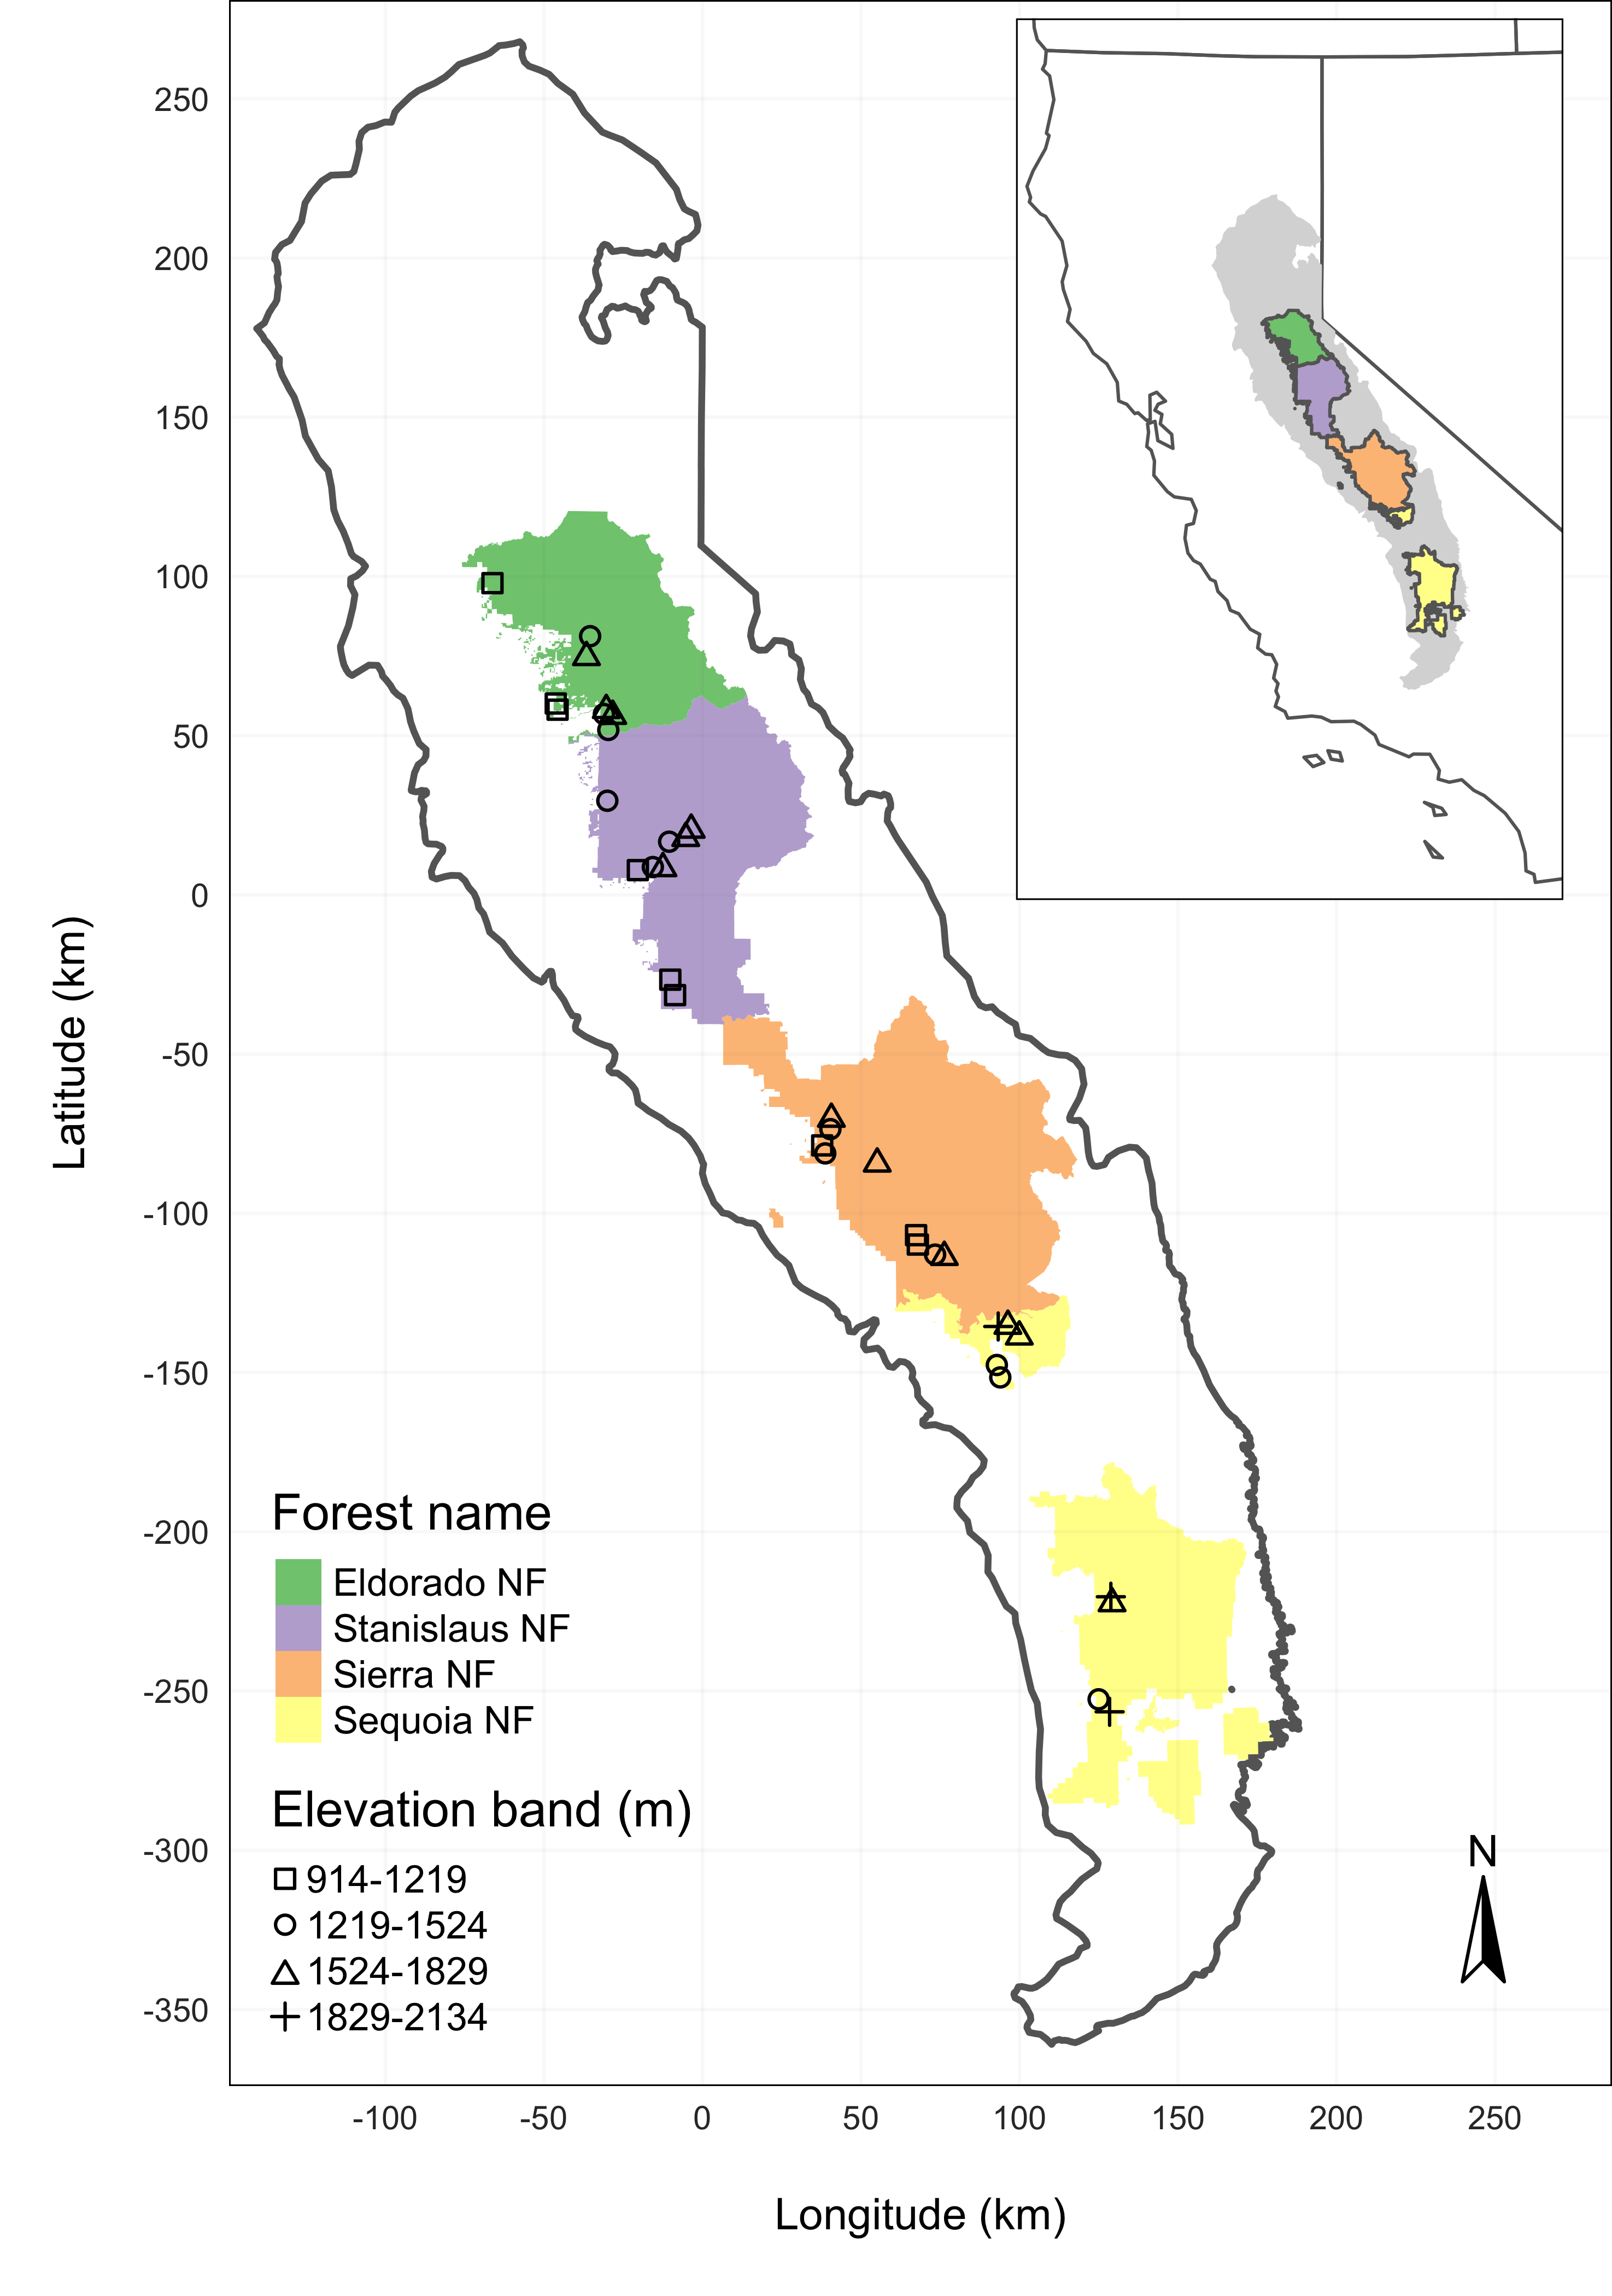
\includegraphics[height=7.00000in]{../../figures/study-geographic-extent-inset.png}
\caption{The network of field plots spanned a 350 km latitudinal
gradient from the Eldorado National Forest in the north to the Sequoia
National Forest in the south. Plots were stratified by three elevation
bands in each forest, with the plots in the Sequoia National Forest (the
southern-most National Forest) occupying elevation bands 305m above the
three bands in the other National Forests in order to capture a similar
community composition.}
\end{figure}

\subsubsection{Instrumentation}\label{instrumentation}

Imagery was captured using a DJI Zenmuse X3 RGB camera (DJI 2015a) and a
Micasense RedEdge3 5-band multispectral camera (Micasense 2015). We
mounted both of these instruments simultaneously on a DJI Matrice 100
aircraft (DJI 2015b) using the DJI 3-axis stabilized gimbal for the
Zenmuse X3 camera and a Micasense angled fixed mount for the RedEdge3
camera. The gimbal and the angled fixed mount ensured both instruments
were nadir-facing during image capture. Just prior or after image
capture at each site, we calibrated the RedEdge3 camera by taking an
image of a calibration panel on the ground in full sun with known
reflectance values for each of the 5 narrow bands.

\begin{longtable}[]{@{}cccccc@{}}
\caption{Reflectance sensitivity of the Micasense Rededge3 camera. The
calibration panel value represents the reflectance of the calibration
panel for the given wavelength.}\tabularnewline
\toprule
\begin{minipage}[b]{0.10\columnwidth}\centering\strut
Band number\strut
\end{minipage} & \begin{minipage}[b]{0.23\columnwidth}\centering\strut
Band name\strut
\end{minipage} & \begin{minipage}[b]{0.14\columnwidth}\centering\strut
Center wavelength\strut
\end{minipage} & \begin{minipage}[b]{0.09\columnwidth}\centering\strut
Band width\strut
\end{minipage} & \begin{minipage}[b]{0.14\columnwidth}\centering\strut
Wavelength range\strut
\end{minipage} & \begin{minipage}[b]{0.14\columnwidth}\centering\strut
Panel reflectance\strut
\end{minipage}\tabularnewline
\midrule
\endfirsthead
\toprule
\begin{minipage}[b]{0.10\columnwidth}\centering\strut
Band number\strut
\end{minipage} & \begin{minipage}[b]{0.23\columnwidth}\centering\strut
Band name\strut
\end{minipage} & \begin{minipage}[b]{0.14\columnwidth}\centering\strut
Center wavelength\strut
\end{minipage} & \begin{minipage}[b]{0.09\columnwidth}\centering\strut
Band width\strut
\end{minipage} & \begin{minipage}[b]{0.14\columnwidth}\centering\strut
Wavelength range\strut
\end{minipage} & \begin{minipage}[b]{0.14\columnwidth}\centering\strut
Panel reflectance\strut
\end{minipage}\tabularnewline
\midrule
\endhead
\begin{minipage}[t]{0.10\columnwidth}\centering\strut
1\strut
\end{minipage} & \begin{minipage}[t]{0.23\columnwidth}\centering\strut
blue (b)\strut
\end{minipage} & \begin{minipage}[t]{0.14\columnwidth}\centering\strut
475\strut
\end{minipage} & \begin{minipage}[t]{0.09\columnwidth}\centering\strut
20\strut
\end{minipage} & \begin{minipage}[t]{0.14\columnwidth}\centering\strut
465-485\strut
\end{minipage} & \begin{minipage}[t]{0.14\columnwidth}\centering\strut
0.64\strut
\end{minipage}\tabularnewline
\begin{minipage}[t]{0.10\columnwidth}\centering\strut
2\strut
\end{minipage} & \begin{minipage}[t]{0.23\columnwidth}\centering\strut
green (g)\strut
\end{minipage} & \begin{minipage}[t]{0.14\columnwidth}\centering\strut
560\strut
\end{minipage} & \begin{minipage}[t]{0.09\columnwidth}\centering\strut
20\strut
\end{minipage} & \begin{minipage}[t]{0.14\columnwidth}\centering\strut
550-570\strut
\end{minipage} & \begin{minipage}[t]{0.14\columnwidth}\centering\strut
0.64\strut
\end{minipage}\tabularnewline
\begin{minipage}[t]{0.10\columnwidth}\centering\strut
3\strut
\end{minipage} & \begin{minipage}[t]{0.23\columnwidth}\centering\strut
red (r)\strut
\end{minipage} & \begin{minipage}[t]{0.14\columnwidth}\centering\strut
668\strut
\end{minipage} & \begin{minipage}[t]{0.09\columnwidth}\centering\strut
10\strut
\end{minipage} & \begin{minipage}[t]{0.14\columnwidth}\centering\strut
663-673\strut
\end{minipage} & \begin{minipage}[t]{0.14\columnwidth}\centering\strut
0.64\strut
\end{minipage}\tabularnewline
\begin{minipage}[t]{0.10\columnwidth}\centering\strut
4\strut
\end{minipage} & \begin{minipage}[t]{0.23\columnwidth}\centering\strut
near infrared (nir)\strut
\end{minipage} & \begin{minipage}[t]{0.14\columnwidth}\centering\strut
840\strut
\end{minipage} & \begin{minipage}[t]{0.09\columnwidth}\centering\strut
40\strut
\end{minipage} & \begin{minipage}[t]{0.14\columnwidth}\centering\strut
820-860\strut
\end{minipage} & \begin{minipage}[t]{0.14\columnwidth}\centering\strut
0.6\strut
\end{minipage}\tabularnewline
\begin{minipage}[t]{0.10\columnwidth}\centering\strut
5\strut
\end{minipage} & \begin{minipage}[t]{0.23\columnwidth}\centering\strut
red edge (re)\strut
\end{minipage} & \begin{minipage}[t]{0.14\columnwidth}\centering\strut
717\strut
\end{minipage} & \begin{minipage}[t]{0.09\columnwidth}\centering\strut
10\strut
\end{minipage} & \begin{minipage}[t]{0.14\columnwidth}\centering\strut
712-722\strut
\end{minipage} & \begin{minipage}[t]{0.14\columnwidth}\centering\strut
0.63\strut
\end{minipage}\tabularnewline
\bottomrule
\end{longtable}

\subsubsection{Flight protocol}\label{flight-protocol}

Image capture was conducted as close to solar noon as possible to
minimize shadow effects (always within 4 hours; usually within 2 hours).
Prior to the aerial survey, two strips of bright orange drop cloth
(\textasciitilde{}100cm x 15cm) were positioned as an ``X'' over the
permanent monuments marking the center of the 5 field plots from Fettig
et al. (2019).

For each of the 36 sites (containing 5 plots each), we captured imagery
over the surrounding \textasciitilde{}40 hectares of forested area using
north-south aerial transects. For three sites, we surveyed less
surrounding area in order to maintain visual and radio communication
with the aircraft during flight which can be obstructed by steep terrain
or non-centrally available takeoff locations. (Table 3; as a supplement,
I think; Columns: Site, forest, elevation, rep, CWD, surveyed area,
survey date).

We preprogrammed transect paths using Map Pilot for DJI on iOS
(hereafter Map Pilot) (Easy 2018). All transects tracked the terrain and
their altitude remained approximately constant at 120 meters above
ground level in order to maintain consistent ground sampling distance in
the imagery. Ground level was based on a 1-arc-second digital elevation
model (Farr et al. 2007) and we implemented terrain following using Map
Pilot. For this analysis, we dropped 4 sites whose imagery was of
insufficient quality to process.

Structure from motion (SfM) processing requires highly overlapping
images, especially in densely vegetated areas. We planned transects with
90\% forward overlap and 90\% side overlap at 100 meters below the lens.
Thus, with flights being at 120 meters above ground level, we achieved
slightly higher than 90/90 overlap for objects 20 meters tall or shorter
(91.6/91.6 overlap at the ground). Overlap values were based on focal
length (3.6mm), sensor width (6.2mm), and image dimension (4000x3000
pixels) parameters of the Zenmuse X3 camera. Images were captured at a
constant rate of 1 image every 2 seconds for both cameras. A forward
overlap of 90\% at 100 meters translates to a flight speed of
approximately 6.45 m/s and a side overlap of 90\% at 100 meters
translates to transects approximately 17.2 meters apart. The Rededge
camera has a different focal length (5.4mm), sensor width (4.8mm), and
image dimension (1280x960 pixels), which translates to image overlap of
80.7/80.7 at 100m below the lens and 83.9/83.9 at ground level.
Approximately 1900 photos were captured over each 40 hectare survey area
for each camera.

\subsubsection{Structure from motion/Photogrammetric
processing}\label{structure-from-motionphotogrammetric-processing}

We used structure from motion (SfM), aka photogrammetry, to generate
orthorectified reflectance maps, digital surface models, and dense point
clouds for each field site. We used Pix4Dmapper Cloud to process imagery
using parameters ideal for images of a densely vegetated area taken by a
multispectral camera. For three sites, we processed the RGB and the
multispectral imagery in the same project to enhance the resolution of
the dense point cloud. All SfM projects resulted in a single processing
``block,'' indicating that all images in the project were optimized and
processed together.

\subsubsection{Creating canopy height
models}\label{creating-canopy-height-models}

We classified each survey area's dense point cloud into ``ground'' and
``non-ground'' points using a cloth simulation filter algorithm (Zhang
et al. 2016) implemented in the \texttt{lidR} (Roussel et al. 2019)
package. We rasterized the ground points using the \texttt{raster}
package (Hijmans et al. 2019) to create a digital terrain model
representing the ground underneath the vegetation at 1 meter resolution.
We created a canopy height model by subtracting the digital terrain
model from the digital surface model created in Pix4Dmapper.

\subsubsection{Tree detection}\label{tree-detection}

We tested a total of 7 automatic tree detection algorithms and a total
of 177 parameter sets on the canopy height model or the dense point
cloud to locate trees within each site (Table 2). We used 3 parameter
sets of a variable window filter implmented in \texttt{ForestTools}
(Plowright 2018) including the default variable window filter function
in \texttt{ForestTools} as well as the ``pines'' and ``combined''
functions from Popescu and Wynne (2004). We used 6 parameter sets of a
local maximum filter implemented in \texttt{lidR}. We used 131 parameter
sets of the algorithm from Li et al. (2012), which operates on the
original point cloud. These parameter sets included those from Shin et
al. (2018) and Jakubowski et al. (2013). We used 3 parameter sets of the
\texttt{watershed} algorithm implemented in \texttt{lidR}, which is a
wrapper for a function in the \texttt{EBImage} package (Pau et al.
2010). We used 3 parameter sets of \texttt{ptrees} (Vega et al. 2014)
implemented in \texttt{lidR} (Roussel et al. 2019) and
\texttt{lidRplugins} (Roussel 2019) and which operates on the raw point
cloud, without first normalizing it to height above ground level (i.e..
subtracting the ground elevation from the dense point cloud). We used
the default parameter set of the \texttt{multichm} (Eysn et al. 2015)
algorithm implmented in \texttt{lidR} (Roussel et al. 2019) and
\texttt{lidRplugins} (Roussel 2019). We used 30 parameter sets of the
experimental algorithm \texttt{lmfx} (Roussel 2019).

\begin{longtable}[]{@{}ccc@{}}
\caption{Algorithm name, number of parameter sets tested for each
algorithm, and references.}\tabularnewline
\toprule
\begin{minipage}[b]{0.18\columnwidth}\centering\strut
Algorithm\strut
\end{minipage} & \begin{minipage}[b]{0.22\columnwidth}\centering\strut
Parameter sets tested\strut
\end{minipage} & \begin{minipage}[b]{0.34\columnwidth}\centering\strut
Reference(s)\strut
\end{minipage}\tabularnewline
\midrule
\endfirsthead
\toprule
\begin{minipage}[b]{0.18\columnwidth}\centering\strut
Algorithm\strut
\end{minipage} & \begin{minipage}[b]{0.22\columnwidth}\centering\strut
Parameter sets tested\strut
\end{minipage} & \begin{minipage}[b]{0.34\columnwidth}\centering\strut
Reference(s)\strut
\end{minipage}\tabularnewline
\midrule
\endhead
\begin{minipage}[t]{0.18\columnwidth}\centering\strut
li2012\strut
\end{minipage} & \begin{minipage}[t]{0.22\columnwidth}\centering\strut
131\strut
\end{minipage} & \begin{minipage}[t]{0.34\columnwidth}\centering\strut
Li et al. (2012); Jakubowski et al. (2013); Shin et al. (2018)\strut
\end{minipage}\tabularnewline
\begin{minipage}[t]{0.18\columnwidth}\centering\strut
lmfx\strut
\end{minipage} & \begin{minipage}[t]{0.22\columnwidth}\centering\strut
30\strut
\end{minipage} & \begin{minipage}[t]{0.34\columnwidth}\centering\strut
Roussel (2019)\strut
\end{minipage}\tabularnewline
\begin{minipage}[t]{0.18\columnwidth}\centering\strut
localMaxima\strut
\end{minipage} & \begin{minipage}[t]{0.22\columnwidth}\centering\strut
6\strut
\end{minipage} & \begin{minipage}[t]{0.34\columnwidth}\centering\strut
Roussel et al. (2019)\strut
\end{minipage}\tabularnewline
\begin{minipage}[t]{0.18\columnwidth}\centering\strut
multichm\strut
\end{minipage} & \begin{minipage}[t]{0.22\columnwidth}\centering\strut
1\strut
\end{minipage} & \begin{minipage}[t]{0.34\columnwidth}\centering\strut
Eysn et al. (2015)\strut
\end{minipage}\tabularnewline
\begin{minipage}[t]{0.18\columnwidth}\centering\strut
ptrees\strut
\end{minipage} & \begin{minipage}[t]{0.22\columnwidth}\centering\strut
3\strut
\end{minipage} & \begin{minipage}[t]{0.34\columnwidth}\centering\strut
Vega et al. (2014)\strut
\end{minipage}\tabularnewline
\begin{minipage}[t]{0.18\columnwidth}\centering\strut
vwf\strut
\end{minipage} & \begin{minipage}[t]{0.22\columnwidth}\centering\strut
3\strut
\end{minipage} & \begin{minipage}[t]{0.34\columnwidth}\centering\strut
Plowright (2018)\strut
\end{minipage}\tabularnewline
\begin{minipage}[t]{0.18\columnwidth}\centering\strut
watershed\strut
\end{minipage} & \begin{minipage}[t]{0.22\columnwidth}\centering\strut
3\strut
\end{minipage} & \begin{minipage}[t]{0.34\columnwidth}\centering\strut
Pau et al. (2010)\strut
\end{minipage}\tabularnewline
\bottomrule
\end{longtable}

\subsubsection{Map ground data}\label{map-ground-data}

Each orthorectified reflectance map was inspected to locate the 5 orange
``X''s marking the center of the field plots. We were able to locate 110
out of 180 field plots and were then able to use these plots for
validation of automated tree detection algorithms. We used the
\texttt{sf} package (Pebesma et al. 2019) to convert
distance-from-center and azimuth measurements of each tree in the ground
plots to an x-y position on the SfM-derived reflectance map using the
x-y position of the orange X visible in the reflectance map as the
center.

\subsubsection{Correspondence of automatic tree detection with ground
data}\label{correspondence-of-automatic-tree-detection-with-ground-data}

We calculated 7 forest structure metrics for each field plot using the
ground data collected by Fettig et al. (2019): total number of trees,
number of trees greater than 15 meters, mean height of trees,
25\textsuperscript{th} percentile tree height, 75\textsuperscript{th}
percentile tree height, mean distance to nearest tree neighbor, mean
distance to 2\textsuperscript{nd} nearest neighbor.

For each tree detection algorithm and parameter set described above, we
calculated the same set of 7 structure metrics within the footprint of
the validation field plots. We calculated the Pearson's correlation and
root mean square error (RMSE) between the ground data and the aerial
data for each of the 7 structure metrics for each of the 177 automatic
tree detection algorithms/parameter sets.

For each algorithm and parameter set, we calculated its performance
relative to other algorithms as whether its Pearson's correlation was
within 5\% of the highest Pearson's correlation as well as whether its
RMSE was within 5\% of the lowest RMSE. For each algorithm/parameter
set, we summed the number of forest structure metrics for which it
reached these 5\% thresholds. For automatically detecting trees across
the whole study, we selected the algorithm/parameter set that performed
well across the most number of forest metrics.

\subsubsection{Segmentation of crowns}\label{segmentation-of-crowns}

We delineated individual tree crowns with a marker controlled watershed
segmentation algorithm (Meyer and Beucher 1990) using the detected
treetops as markers implemented in the \texttt{ForestTools} package
(Plowright 2018). If the automatic segmentation algorithm failed to
generate a crown segment for a detected tree (e.g., often snags with a
very small crown footprint), a circular crown was generated with a
radius of 0.5 meters. If the segmentation generated multiple polygons
for a single detected tree, only the polygon containing the detected
tree was retained. Image overlap decreases near the edges of the overall
flight path, which reduces the quality of the SfM processing in those
areas. Thus, we excluded segmented crowns within 35 meters of the edge
of the survey area. Given the narrower field of view of the RedEdge
multispectral camera versus the X3 RGB camera whose optical parameters
were used to define the \textasciitilde{}40 hectare survey area around
each site, as well as the 35 meter additional buffering, the survey area
at each site was approximately 30 hectares (Table 3).

We used the \texttt{velox} package (Hunziker 2017) to extract all the
pixel values from the orthorectified reflectance map for each of the 5
narrow bands within each segmented crown polygon. Per pixel, we
additionally calculated the normalized difference vegetation index
(NDVI; Rouse et al. (1973)), the normalized difference red edge (NDRE;
Gitelson and Merzlyak (1994)), the red-green index (RGI; Coops et al.
(2006)), the red edge chlorophyll index (CI{[}red edge{]}; Clevers and
Gitelson (2013)), and the green chlorophyll index (CI{[}green{]};
Clevers and Gitelson (2013)). For each crown polygon, we calculated the
mean value for each raw and derived reflectance band (5 raw; 5 derived).

\subsubsection{Classification of trees}\label{classification-of-trees}

We overlaid the segmented crowns on the reflectance maps from 20 sites
spanning the latitudinal and elevational gradient in the study. Using
QGIS, we hand classified 564 trees as live/dead and as one of 5 dominant
species in the study area (\emph{Pinus ponderosa}, \emph{Pinus
lambertiana}, \emph{Abies concolor}, \emph{Calocedrus decurrens}, or
\emph{Quercus kelloggi}) using the mapped ground data as a guide.

We used all 10 mean values of the reflectance bands for each tree crown
polygon to predict whether the hand classified trees were alive or dead
using a boosted logistic regression model implemented in the
\texttt{caret} package (accuracy of live/dead classification on a
witheld test dataset: 97.3\%) (Kuhn 2008). For just the living trees, we
similarly used all 10 reflectance values to predict the tree species
using regularized discriminant analysis implemented in the
\texttt{caret} package (accuracy of species classification on a witheld
testing dataset: 66.7\%; accuracy of WPB host/non-WPB-host (i.e.,
ponderosa pine versus other tree species) on a witheld testing dataset:
74.4\%).

Finally, we used these models to classify all tree crowns in the data
set as alive or dead as well as the species of living trees.

\subsubsection{Allometric scaling of height to basal
area}\label{allometric-scaling-of-height-to-basal-area}

We converted the height of each tree determined using the canopy height
model to its basal area. Using the tree height and diameter at breast
height (DBH; breast height = 1.37m) ground data from Fettig et al.
(2019), we fit a simple linear regression to predict DBH from height for
each of the 5 dominant species. Using the model-classified tree species
of each segmented tree, we used the corresponding linear relationship
for that species to estimate the DBH given the tree's height. We then
calculated each tree's basal area, assuming no tapering from breast
height.

\subsubsection{Note on assumptions about dead
trees}\label{note-on-assumptions-about-dead-trees}

For the purposes of this study, we assumed that all dead trees were
ponderosa pine and were thus host trees for the western pine beetle.
This is a reasonably good assumption, given that Fettig et al. (2019)
found that 73.4\% of the dead trees in the coincident ground plots were
ponderosa pine. The species contributing to the next highest proportion
of dead trees was incense cedar which represented 18.72\% of the dead
trees in the ground plots. Incense cedar is not a potential host of the
western pine beetle, and we expand on the limitations of this study
given the assumption of dead trees being ponderosa pine in the
Discussion.

\subsubsection{Rasterizing individual tree
data}\label{rasterizing-individual-tree-data}

Because the tree detection algorithms were validated against ground data
at the plot level, we rasterized the classified trees at a spatial
resolution similar to that of the ground plots (rasterized to 20m x 20m
equalling 400 m\textsuperscript{2}; circular ground plots with 11.35m
radius equalling 404 m\textsuperscript{2}). In each raster cell, we
calculated the: number of live trees, number of dead trees, number of
ponderosa pine trees, total number of trees (of all species, including
ponderosa pine), quadratic mean diameter (QMD) of ponderosa pine trees,
and QMD of all trees of any species (overall QMD). We converted the
count of ponderosa pine trees and the total tree count to a density
measurement of trees per hectare (tpha) by multiplying the counts in
each 20m x 20m cell by 25 to create a ``host density'' and an ``overall
density'' variable per cell.

\subsubsection{Environmental data}\label{environmental-data}

We used climatic water deficit (CWD) (Stephenson 1998) from the
1980-2010 mean value of the basin characterization model (Flint et al.
2013) as an integrated measure of temperature and moisture conditions
for each cell. Higher values of CWD correspond to hotter, drier
conditions and lower values correspond to cooler, wetter conditions CWD
has been shown to correlate well with broad patterns of tree mortality
in the Sierra Nevada (Young et al. 2017). We resampled the climatic
water deficit product using bilinear interpolation implemented in the
\texttt{raster} package to match the 20m x 20m spatial scale of the
other variables. We converted the CWD value for each cell into a z-score
representing that cell's deviation from the mean CWD across the climatic
range of Sierra Nevada ponderosa pine as determined from 179 herbarium
records described in Baldwin et al. (2017). Thus, a CWD z-score of one
would indicate that the CWD at that cell is one standard deviation
hotter/drier than the mean CWD across all geolocated herbarium records
for ponderosa pine in the Sierra Nevada.

\subsubsection{Statistical model}\label{statistical-model}

We used a generalized linear model with a zero-inflated binomial
response and a logit link to predict the probability of ponderosa pine
mortality within each raster cell as a function of the crossed effects
of ponderosa pine quadratic mean diameter and density added to the
crossed effect of overall quadratic mean diameter and density as well as
the interaction of each summand with climatic water deficit at each
site.

To measure and account for spatial autocorrelation of the bark beetle
behavioral processes underlying ponderosa mortality, we first subsampled
the data at each site to a random selection of 200, 20m x 20m cells
representing approximately 27.5\% of the surveyed area. With these
subsampled data, we included a separate exact Gaussian process term per
site of the interaction between the x- and y-position of each cell using
the \texttt{gp()} function in the \texttt{brms} package (Bürkner 2017).
The Gaussian process accounts for spatial autocorrelation in the model
by jointly estimating the spatial covariance of the response variable
with the effects of the other covariates.

\[
\begin{aligned}
y_{i,j} \sim &\ \begin{cases}
0, & p \\
Binom(n_i, \pi_i), & 1-p
\end{cases} \\
logit(\pi_i) = &\ \beta_0\ + \\
& \beta_1X_{cwd, j}\ + \\
& \beta_1X_{cwd, j}(\beta_2X_{pipoQMD, i} + \beta_3X_{pipoDensity, i} + \beta_4X_{pipoQMD, i}X_{pipoDensity, i})\ + \\ 
& \beta_1X_{cwd, j}(\beta_5X_{overallQMD, i} + \beta_6X_{overallDensity, i} + \beta_7X_{overallQMD, i}X_{overallDensity, i})\ + \\
& \mathcal{GP}_j(x_i, y_i) \\
\end{aligned}
\]

Where \(y_i\) is the number of dead trees in cell \(i\), \(n_i\) is the
sum of the dead trees and live ponderosa pine trees in cell \(i\),
\(\pi_i\) is the probability of ponderosa pine tree mortality in cell
\(i\), \(p\) is the probability of there being zero dead trees in a cell
arising as a result of an unmodeled process, \(X_{cwd, j}\) is the
z-score of climatic water deficit for site \(j\), \(X_{pipoQMD, i}\) is
the scaled quadratic mean diameter of ponderosa pine in cell \(i\),
\(X_{pipoDensity, i}\) is the scaled density of ponderosa pine trees in
cell \(i\), \(X_{overallQMD, i}\) is the scaled quadratic mean diameter
of all trees in cell \(i\), \(X_{overallDensity, i}\) is the scaled
density of all trees in cell \(i\), \(x_i\) and \(y_i\) are the x- and
y- coordinates of the centroid of the cell in an EPSG3310 coordinate
reference system, and \(\mathcal{GP}_j\) represents the exact Gaussian
process describing the spatial covariance between cells at site \(j\).

We used 4 chains with 2000 iterations each (1000 warmup, 1000 samples),
and confirmed chain convergence by ensuring all \texttt{Rhat} values
were less than 1.1 (Brooks and Gelman 1998). We used posterior
predictive checks to visually confirm model performance by overlaying
the density curves of the predicted number of dead trees per cell over
the observed number (Gabry et al. 2019). For the posterior predictive
checks, we used 50 random samples from the model fit to generate 50
density curves and ensured curves were centered on the observed
distribution, paying special attention to model performance at capturing
counts of zero.

\subsubsection{Software and data
availability}\label{software-and-data-availability}

All data are available via the Open Science Framework. Statistical
analyses were performed using the \texttt{brms} packages. With the
exception of the SfM software (Pix4Dmapper Cloud) and the GIS software
QGIS, all data carpentry and analyses were performed using \texttt{R} (R
Core Team 2018).

\subsection{Results}\label{results}

\begin{longtable}[]{@{}cccccc@{}}
\caption{Site characteristics for each of the 32 sites. The site name
consists of the forest name, elevation band, and rep separated by an
underscore. The Eldorado National Forest is `eldo', the Stanislaus
National Forest is `stan', the Sierra National Forest is `sier', and the
Sequoia National Forest is `sequ'. The elevation band represents the
lower bounds of the 305 meter (1000 foot) elevation bands in feet. Thus
`3k' implies that site was located between 3,000 and 4,000 feet
(914-1219 meters). Aerially detected mortality and density of the whole
site is presented along with the mortality and density calculated from
the ground data (aerial / ground). The density is measured in trees per
hectare (tpha).}\tabularnewline
\toprule
\begin{minipage}[b]{0.12\columnwidth}\centering\strut
Site\strut
\end{minipage} & \begin{minipage}[b]{0.07\columnwidth}\centering\strut
CWD (mm)\strut
\end{minipage} & \begin{minipage}[b]{0.12\columnwidth}\centering\strut
CWD (z-score)\strut
\end{minipage} & \begin{minipage}[b]{0.14\columnwidth}\centering\strut
Survey area (ha)\strut
\end{minipage} & \begin{minipage}[b]{0.17\columnwidth}\centering\strut
Mortality (aerial/ground)\strut
\end{minipage} & \begin{minipage}[b]{0.22\columnwidth}\centering\strut
Density (tpha; aerial/ground)\strut
\end{minipage}\tabularnewline
\midrule
\endfirsthead
\toprule
\begin{minipage}[b]{0.12\columnwidth}\centering\strut
Site\strut
\end{minipage} & \begin{minipage}[b]{0.07\columnwidth}\centering\strut
CWD (mm)\strut
\end{minipage} & \begin{minipage}[b]{0.12\columnwidth}\centering\strut
CWD (z-score)\strut
\end{minipage} & \begin{minipage}[b]{0.14\columnwidth}\centering\strut
Survey area (ha)\strut
\end{minipage} & \begin{minipage}[b]{0.17\columnwidth}\centering\strut
Mortality (aerial/ground)\strut
\end{minipage} & \begin{minipage}[b]{0.22\columnwidth}\centering\strut
Density (tpha; aerial/ground)\strut
\end{minipage}\tabularnewline
\midrule
\endhead
\begin{minipage}[t]{0.12\columnwidth}\centering\strut
eldo\_3k\_1\strut
\end{minipage} & \begin{minipage}[t]{0.07\columnwidth}\centering\strut
678\strut
\end{minipage} & \begin{minipage}[t]{0.12\columnwidth}\centering\strut
0.319\strut
\end{minipage} & \begin{minipage}[t]{0.14\columnwidth}\centering\strut
31.02\strut
\end{minipage} & \begin{minipage}[t]{0.17\columnwidth}\centering\strut
0.11/0.61\strut
\end{minipage} & \begin{minipage}[t]{0.22\columnwidth}\centering\strut
630.01/410.19\strut
\end{minipage}\tabularnewline
\begin{minipage}[t]{0.12\columnwidth}\centering\strut
eldo\_3k\_2\strut
\end{minipage} & \begin{minipage}[t]{0.07\columnwidth}\centering\strut
706\strut
\end{minipage} & \begin{minipage}[t]{0.12\columnwidth}\centering\strut
0.501\strut
\end{minipage} & \begin{minipage}[t]{0.14\columnwidth}\centering\strut
30.61\strut
\end{minipage} & \begin{minipage}[t]{0.17\columnwidth}\centering\strut
0.12/0.36\strut
\end{minipage} & \begin{minipage}[t]{0.22\columnwidth}\centering\strut
444.26/647.42\strut
\end{minipage}\tabularnewline
\begin{minipage}[t]{0.12\columnwidth}\centering\strut
eldo\_3k\_3\strut
\end{minipage} & \begin{minipage}[t]{0.07\columnwidth}\centering\strut
655\strut
\end{minipage} & \begin{minipage}[t]{0.12\columnwidth}\centering\strut
0.163\strut
\end{minipage} & \begin{minipage}[t]{0.14\columnwidth}\centering\strut
30.95\strut
\end{minipage} & \begin{minipage}[t]{0.17\columnwidth}\centering\strut
0.22/0.36\strut
\end{minipage} & \begin{minipage}[t]{0.22\columnwidth}\centering\strut
492.63/410.19\strut
\end{minipage}\tabularnewline
\begin{minipage}[t]{0.12\columnwidth}\centering\strut
eldo\_4k\_1\strut
\end{minipage} & \begin{minipage}[t]{0.07\columnwidth}\centering\strut
570\strut
\end{minipage} & \begin{minipage}[t]{0.12\columnwidth}\centering\strut
-0.383\strut
\end{minipage} & \begin{minipage}[t]{0.14\columnwidth}\centering\strut
28.04\strut
\end{minipage} & \begin{minipage}[t]{0.17\columnwidth}\centering\strut
0.09/0.39\strut
\end{minipage} & \begin{minipage}[t]{0.22\columnwidth}\centering\strut
632.82/588.11\strut
\end{minipage}\tabularnewline
\begin{minipage}[t]{0.12\columnwidth}\centering\strut
eldo\_4k\_2\strut
\end{minipage} & \begin{minipage}[t]{0.07\columnwidth}\centering\strut
642\strut
\end{minipage} & \begin{minipage}[t]{0.12\columnwidth}\centering\strut
0.0831\strut
\end{minipage} & \begin{minipage}[t]{0.14\columnwidth}\centering\strut
28.41\strut
\end{minipage} & \begin{minipage}[t]{0.17\columnwidth}\centering\strut
0.15/0.78\strut
\end{minipage} & \begin{minipage}[t]{0.22\columnwidth}\centering\strut
338.20/271.82\strut
\end{minipage}\tabularnewline
\begin{minipage}[t]{0.12\columnwidth}\centering\strut
eldo\_5k\_1\strut
\end{minipage} & \begin{minipage}[t]{0.07\columnwidth}\centering\strut
663\strut
\end{minipage} & \begin{minipage}[t]{0.12\columnwidth}\centering\strut
0.219\strut
\end{minipage} & \begin{minipage}[t]{0.14\columnwidth}\centering\strut
28.44\strut
\end{minipage} & \begin{minipage}[t]{0.17\columnwidth}\centering\strut
0.11/0.44\strut
\end{minipage} & \begin{minipage}[t]{0.22\columnwidth}\centering\strut
661.80/543.63\strut
\end{minipage}\tabularnewline
\begin{minipage}[t]{0.12\columnwidth}\centering\strut
eldo\_5k\_2\strut
\end{minipage} & \begin{minipage}[t]{0.07\columnwidth}\centering\strut
627\strut
\end{minipage} & \begin{minipage}[t]{0.12\columnwidth}\centering\strut
-0.0132\strut
\end{minipage} & \begin{minipage}[t]{0.14\columnwidth}\centering\strut
30.02\strut
\end{minipage} & \begin{minipage}[t]{0.17\columnwidth}\centering\strut
0.12/0.36\strut
\end{minipage} & \begin{minipage}[t]{0.22\columnwidth}\centering\strut
584.89/968.65\strut
\end{minipage}\tabularnewline
\begin{minipage}[t]{0.12\columnwidth}\centering\strut
eldo\_5k\_3\strut
\end{minipage} & \begin{minipage}[t]{0.07\columnwidth}\centering\strut
599\strut
\end{minipage} & \begin{minipage}[t]{0.12\columnwidth}\centering\strut
-0.2\strut
\end{minipage} & \begin{minipage}[t]{0.14\columnwidth}\centering\strut
29.73\strut
\end{minipage} & \begin{minipage}[t]{0.17\columnwidth}\centering\strut
0.07/0.32\strut
\end{minipage} & \begin{minipage}[t]{0.22\columnwidth}\centering\strut
488.66/622.71\strut
\end{minipage}\tabularnewline
\begin{minipage}[t]{0.12\columnwidth}\centering\strut
stan\_3k\_1\strut
\end{minipage} & \begin{minipage}[t]{0.07\columnwidth}\centering\strut
638\strut
\end{minipage} & \begin{minipage}[t]{0.12\columnwidth}\centering\strut
0.059\strut
\end{minipage} & \begin{minipage}[t]{0.14\columnwidth}\centering\strut
31.04\strut
\end{minipage} & \begin{minipage}[t]{0.17\columnwidth}\centering\strut
0.10/0.52\strut
\end{minipage} & \begin{minipage}[t]{0.22\columnwidth}\centering\strut
739.45/1037.84\strut
\end{minipage}\tabularnewline
\begin{minipage}[t]{0.12\columnwidth}\centering\strut
stan\_3k\_2\strut
\end{minipage} & \begin{minipage}[t]{0.07\columnwidth}\centering\strut
739\strut
\end{minipage} & \begin{minipage}[t]{0.12\columnwidth}\centering\strut
0.713\strut
\end{minipage} & \begin{minipage}[t]{0.14\columnwidth}\centering\strut
18.78\strut
\end{minipage} & \begin{minipage}[t]{0.17\columnwidth}\centering\strut
0.40/0.78\strut
\end{minipage} & \begin{minipage}[t]{0.22\columnwidth}\centering\strut
433.53/405.25\strut
\end{minipage}\tabularnewline
\begin{minipage}[t]{0.12\columnwidth}\centering\strut
stan\_3k\_3\strut
\end{minipage} & \begin{minipage}[t]{0.07\columnwidth}\centering\strut
762\strut
\end{minipage} & \begin{minipage}[t]{0.12\columnwidth}\centering\strut
0.859\strut
\end{minipage} & \begin{minipage}[t]{0.14\columnwidth}\centering\strut
30.1\strut
\end{minipage} & \begin{minipage}[t]{0.17\columnwidth}\centering\strut
0.22/0.41\strut
\end{minipage} & \begin{minipage}[t]{0.22\columnwidth}\centering\strut
558.43/326.18\strut
\end{minipage}\tabularnewline
\begin{minipage}[t]{0.12\columnwidth}\centering\strut
stan\_4k\_1\strut
\end{minipage} & \begin{minipage}[t]{0.07\columnwidth}\centering\strut
540\strut
\end{minipage} & \begin{minipage}[t]{0.12\columnwidth}\centering\strut
-0.58\strut
\end{minipage} & \begin{minipage}[t]{0.14\columnwidth}\centering\strut
29.62\strut
\end{minipage} & \begin{minipage}[t]{0.17\columnwidth}\centering\strut
0.29/0.63\strut
\end{minipage} & \begin{minipage}[t]{0.22\columnwidth}\centering\strut
507.61/711.66\strut
\end{minipage}\tabularnewline
\begin{minipage}[t]{0.12\columnwidth}\centering\strut
stan\_4k\_2\strut
\end{minipage} & \begin{minipage}[t]{0.07\columnwidth}\centering\strut
528\strut
\end{minipage} & \begin{minipage}[t]{0.12\columnwidth}\centering\strut
-0.658\strut
\end{minipage} & \begin{minipage}[t]{0.14\columnwidth}\centering\strut
30.54\strut
\end{minipage} & \begin{minipage}[t]{0.17\columnwidth}\centering\strut
0.18/0.56\strut
\end{minipage} & \begin{minipage}[t]{0.22\columnwidth}\centering\strut
481.85/256.99\strut
\end{minipage}\tabularnewline
\begin{minipage}[t]{0.12\columnwidth}\centering\strut
stan\_5k\_1\strut
\end{minipage} & \begin{minipage}[t]{0.07\columnwidth}\centering\strut
524\strut
\end{minipage} & \begin{minipage}[t]{0.12\columnwidth}\centering\strut
-0.688\strut
\end{minipage} & \begin{minipage}[t]{0.14\columnwidth}\centering\strut
30.94\strut
\end{minipage} & \begin{minipage}[t]{0.17\columnwidth}\centering\strut
0.19/0.54\strut
\end{minipage} & \begin{minipage}[t]{0.22\columnwidth}\centering\strut
388.89/336.06\strut
\end{minipage}\tabularnewline
\begin{minipage}[t]{0.12\columnwidth}\centering\strut
stan\_5k\_2\strut
\end{minipage} & \begin{minipage}[t]{0.07\columnwidth}\centering\strut
524\strut
\end{minipage} & \begin{minipage}[t]{0.12\columnwidth}\centering\strut
-0.685\strut
\end{minipage} & \begin{minipage}[t]{0.14\columnwidth}\centering\strut
29.94\strut
\end{minipage} & \begin{minipage}[t]{0.17\columnwidth}\centering\strut
0.21/0.44\strut
\end{minipage} & \begin{minipage}[t]{0.22\columnwidth}\centering\strut
399.33/622.71\strut
\end{minipage}\tabularnewline
\begin{minipage}[t]{0.12\columnwidth}\centering\strut
sier\_3k\_1\strut
\end{minipage} & \begin{minipage}[t]{0.07\columnwidth}\centering\strut
764\strut
\end{minipage} & \begin{minipage}[t]{0.12\columnwidth}\centering\strut
0.871\strut
\end{minipage} & \begin{minipage}[t]{0.14\columnwidth}\centering\strut
30.42\strut
\end{minipage} & \begin{minipage}[t]{0.17\columnwidth}\centering\strut
0.19/0.48\strut
\end{minipage} & \begin{minipage}[t]{0.22\columnwidth}\centering\strut
651.46/850.04\strut
\end{minipage}\tabularnewline
\begin{minipage}[t]{0.12\columnwidth}\centering\strut
sier\_3k\_2\strut
\end{minipage} & \begin{minipage}[t]{0.07\columnwidth}\centering\strut
768\strut
\end{minipage} & \begin{minipage}[t]{0.12\columnwidth}\centering\strut
0.898\strut
\end{minipage} & \begin{minipage}[t]{0.14\columnwidth}\centering\strut
30.05\strut
\end{minipage} & \begin{minipage}[t]{0.17\columnwidth}\centering\strut
0.20/0.77\strut
\end{minipage} & \begin{minipage}[t]{0.22\columnwidth}\centering\strut
438.84/153.21\strut
\end{minipage}\tabularnewline
\begin{minipage}[t]{0.12\columnwidth}\centering\strut
sier\_3k\_3\strut
\end{minipage} & \begin{minipage}[t]{0.07\columnwidth}\centering\strut
773\strut
\end{minipage} & \begin{minipage}[t]{0.12\columnwidth}\centering\strut
0.932\strut
\end{minipage} & \begin{minipage}[t]{0.14\columnwidth}\centering\strut
29.77\strut
\end{minipage} & \begin{minipage}[t]{0.17\columnwidth}\centering\strut
0.32/0.77\strut
\end{minipage} & \begin{minipage}[t]{0.22\columnwidth}\centering\strut
511.26/459.62\strut
\end{minipage}\tabularnewline
\begin{minipage}[t]{0.12\columnwidth}\centering\strut
sier\_4k\_1\strut
\end{minipage} & \begin{minipage}[t]{0.07\columnwidth}\centering\strut
841\strut
\end{minipage} & \begin{minipage}[t]{0.12\columnwidth}\centering\strut
1.38\strut
\end{minipage} & \begin{minipage}[t]{0.14\columnwidth}\centering\strut
30.43\strut
\end{minipage} & \begin{minipage}[t]{0.17\columnwidth}\centering\strut
0.54/0.51\strut
\end{minipage} & \begin{minipage}[t]{0.22\columnwidth}\centering\strut
576.15/538.69\strut
\end{minipage}\tabularnewline
\begin{minipage}[t]{0.12\columnwidth}\centering\strut
sier\_4k\_2\strut
\end{minipage} & \begin{minipage}[t]{0.07\columnwidth}\centering\strut
764\strut
\end{minipage} & \begin{minipage}[t]{0.12\columnwidth}\centering\strut
0.877\strut
\end{minipage} & \begin{minipage}[t]{0.14\columnwidth}\centering\strut
29.3\strut
\end{minipage} & \begin{minipage}[t]{0.17\columnwidth}\centering\strut
0.33/0.57\strut
\end{minipage} & \begin{minipage}[t]{0.22\columnwidth}\centering\strut
499.43/854.98\strut
\end{minipage}\tabularnewline
\begin{minipage}[t]{0.12\columnwidth}\centering\strut
sier\_4k\_3\strut
\end{minipage} & \begin{minipage}[t]{0.07\columnwidth}\centering\strut
688\strut
\end{minipage} & \begin{minipage}[t]{0.12\columnwidth}\centering\strut
0.383\strut
\end{minipage} & \begin{minipage}[t]{0.14\columnwidth}\centering\strut
26.39\strut
\end{minipage} & \begin{minipage}[t]{0.17\columnwidth}\centering\strut
0.48/0.59\strut
\end{minipage} & \begin{minipage}[t]{0.22\columnwidth}\centering\strut
454.23/499.15\strut
\end{minipage}\tabularnewline
\begin{minipage}[t]{0.12\columnwidth}\centering\strut
sier\_5k\_1\strut
\end{minipage} & \begin{minipage}[t]{0.07\columnwidth}\centering\strut
722\strut
\end{minipage} & \begin{minipage}[t]{0.12\columnwidth}\centering\strut
0.599\strut
\end{minipage} & \begin{minipage}[t]{0.14\columnwidth}\centering\strut
14.59\strut
\end{minipage} & \begin{minipage}[t]{0.17\columnwidth}\centering\strut
0.41/0.43\strut
\end{minipage} & \begin{minipage}[t]{0.22\columnwidth}\centering\strut
631.30/716.60\strut
\end{minipage}\tabularnewline
\begin{minipage}[t]{0.12\columnwidth}\centering\strut
sier\_5k\_2\strut
\end{minipage} & \begin{minipage}[t]{0.07\columnwidth}\centering\strut
710\strut
\end{minipage} & \begin{minipage}[t]{0.12\columnwidth}\centering\strut
0.523\strut
\end{minipage} & \begin{minipage}[t]{0.14\columnwidth}\centering\strut
27.53\strut
\end{minipage} & \begin{minipage}[t]{0.17\columnwidth}\centering\strut
0.53/0.74\strut
\end{minipage} & \begin{minipage}[t]{0.22\columnwidth}\centering\strut
477.29/454.67\strut
\end{minipage}\tabularnewline
\begin{minipage}[t]{0.12\columnwidth}\centering\strut
sier\_5k\_3\strut
\end{minipage} & \begin{minipage}[t]{0.07\columnwidth}\centering\strut
779\strut
\end{minipage} & \begin{minipage}[t]{0.12\columnwidth}\centering\strut
0.968\strut
\end{minipage} & \begin{minipage}[t]{0.14\columnwidth}\centering\strut
28.93\strut
\end{minipage} & \begin{minipage}[t]{0.17\columnwidth}\centering\strut
0.33/0.43\strut
\end{minipage} & \begin{minipage}[t]{0.22\columnwidth}\centering\strut
569.44/484.33\strut
\end{minipage}\tabularnewline
\begin{minipage}[t]{0.12\columnwidth}\centering\strut
sequ\_4k\_1\strut
\end{minipage} & \begin{minipage}[t]{0.07\columnwidth}\centering\strut
767\strut
\end{minipage} & \begin{minipage}[t]{0.12\columnwidth}\centering\strut
0.891\strut
\end{minipage} & \begin{minipage}[t]{0.14\columnwidth}\centering\strut
29.59\strut
\end{minipage} & \begin{minipage}[t]{0.17\columnwidth}\centering\strut
0.50/0.56\strut
\end{minipage} & \begin{minipage}[t]{0.22\columnwidth}\centering\strut
365.81/607.88\strut
\end{minipage}\tabularnewline
\begin{minipage}[t]{0.12\columnwidth}\centering\strut
sequ\_4k\_3\strut
\end{minipage} & \begin{minipage}[t]{0.07\columnwidth}\centering\strut
816\strut
\end{minipage} & \begin{minipage}[t]{0.12\columnwidth}\centering\strut
1.21\strut
\end{minipage} & \begin{minipage}[t]{0.14\columnwidth}\centering\strut
29.69\strut
\end{minipage} & \begin{minipage}[t]{0.17\columnwidth}\centering\strut
0.35/0.71\strut
\end{minipage} & \begin{minipage}[t]{0.22\columnwidth}\centering\strut
433.35/306.41\strut
\end{minipage}\tabularnewline
\begin{minipage}[t]{0.12\columnwidth}\centering\strut
sequ\_5k\_1\strut
\end{minipage} & \begin{minipage}[t]{0.07\columnwidth}\centering\strut
718\strut
\end{minipage} & \begin{minipage}[t]{0.12\columnwidth}\centering\strut
0.577\strut
\end{minipage} & \begin{minipage}[t]{0.14\columnwidth}\centering\strut
27.12\strut
\end{minipage} & \begin{minipage}[t]{0.17\columnwidth}\centering\strut
0.35/0.52\strut
\end{minipage} & \begin{minipage}[t]{0.22\columnwidth}\centering\strut
364.01/444.79\strut
\end{minipage}\tabularnewline
\begin{minipage}[t]{0.12\columnwidth}\centering\strut
sequ\_5k\_2\strut
\end{minipage} & \begin{minipage}[t]{0.07\columnwidth}\centering\strut
587\strut
\end{minipage} & \begin{minipage}[t]{0.12\columnwidth}\centering\strut
-0.274\strut
\end{minipage} & \begin{minipage}[t]{0.14\columnwidth}\centering\strut
29.1\strut
\end{minipage} & \begin{minipage}[t]{0.17\columnwidth}\centering\strut
0.45/0.43\strut
\end{minipage} & \begin{minipage}[t]{0.22\columnwidth}\centering\strut
478.31/499.15\strut
\end{minipage}\tabularnewline
\begin{minipage}[t]{0.12\columnwidth}\centering\strut
sequ\_5k\_3\strut
\end{minipage} & \begin{minipage}[t]{0.07\columnwidth}\centering\strut
611\strut
\end{minipage} & \begin{minipage}[t]{0.12\columnwidth}\centering\strut
-0.117\strut
\end{minipage} & \begin{minipage}[t]{0.14\columnwidth}\centering\strut
31.34\strut
\end{minipage} & \begin{minipage}[t]{0.17\columnwidth}\centering\strut
0.42/0.48\strut
\end{minipage} & \begin{minipage}[t]{0.22\columnwidth}\centering\strut
348.68/494.21\strut
\end{minipage}\tabularnewline
\begin{minipage}[t]{0.12\columnwidth}\centering\strut
sequ\_6k\_1\strut
\end{minipage} & \begin{minipage}[t]{0.07\columnwidth}\centering\strut
731\strut
\end{minipage} & \begin{minipage}[t]{0.12\columnwidth}\centering\strut
0.657\strut
\end{minipage} & \begin{minipage}[t]{0.14\columnwidth}\centering\strut
27.78\strut
\end{minipage} & \begin{minipage}[t]{0.17\columnwidth}\centering\strut
0.30/0.70\strut
\end{minipage} & \begin{minipage}[t]{0.22\columnwidth}\centering\strut
433.43/360.77\strut
\end{minipage}\tabularnewline
\begin{minipage}[t]{0.12\columnwidth}\centering\strut
sequ\_6k\_2\strut
\end{minipage} & \begin{minipage}[t]{0.07\columnwidth}\centering\strut
690\strut
\end{minipage} & \begin{minipage}[t]{0.12\columnwidth}\centering\strut
0.39\strut
\end{minipage} & \begin{minipage}[t]{0.14\columnwidth}\centering\strut
11.83\strut
\end{minipage} & \begin{minipage}[t]{0.17\columnwidth}\centering\strut
0.26/0.43\strut
\end{minipage} & \begin{minipage}[t]{0.22\columnwidth}\centering\strut
699.04/934.06\strut
\end{minipage}\tabularnewline
\begin{minipage}[t]{0.12\columnwidth}\centering\strut
sequ\_6k\_3\strut
\end{minipage} & \begin{minipage}[t]{0.07\columnwidth}\centering\strut
603\strut
\end{minipage} & \begin{minipage}[t]{0.12\columnwidth}\centering\strut
-0.174\strut
\end{minipage} & \begin{minipage}[t]{0.14\columnwidth}\centering\strut
26.51\strut
\end{minipage} & \begin{minipage}[t]{0.17\columnwidth}\centering\strut
0.36/0.32\strut
\end{minipage} & \begin{minipage}[t]{0.22\columnwidth}\centering\strut
535.54/691.89\strut
\end{minipage}\tabularnewline
\bottomrule
\end{longtable}

\begin{figure}
\centering
\includegraphics{../../figures/eldo_3k_3_point_cloud.png}
\caption{A dense point cloud representing \textasciitilde{}40 hectares
of forest is generated using Structure from Motion (SfM) processing of
\textasciitilde{}1900 images. The dense point cloud z- position
represents the ground elevation plus the vegetation height.}
\end{figure}

\begin{figure}
\centering

\includegraphics{../../figures/eldo_3k_3_dsm.png}
\caption{The digital surface model (DSM) is a 2-dimensional
representation of the dense point cloud generated using structure from
motion (SfM) processing. The DSM represents the ground elevation plus
the vegetation height.}
\end{figure}

\begin{figure}
\centering
\includegraphics{../../figures/eldo_3k_3_dtm.png}
\caption{The digital terrain model (DTM) is generated by processing the
dense point cloud using the cloth simulation filter algorithm (Zhang et
al. 2016), which classifies points as ``ground'' or ``not-ground'' and
then interpolates the ``ground'' elevation using Delaunay triangulation
for the rest of the dense point cloud footprint. The DTM represents the
ground elevation without any vegetation.}
\end{figure}

\begin{figure}
\centering
\includegraphics{../../figures/eldo_3k_3_chm.png}
\caption{The canopy height model (CHM) is generated by subtracting the
digital terrain model from the digital surface model. The CHM represents
the height of all of the elevation above ground level.}
\end{figure}

\begin{figure}
\centering
\includegraphics{../../figures/eldo_3k_3_ttops.png}
\caption{Tree locations are detected using the \texttt{lmfx} (Roussel et
al. 2019) treetop detection algorithm on the dense point cloud.}
\end{figure}

\begin{figure}
\centering
\includegraphics{../../figures/eldo_3k_3_crowns.png}
\caption{Individual crowns are delineated using a marker controlled
watershed segmentation algorithm (Meyer and Beucher 1990, Plowright
2018) on the canopy height model (CHM) using the detected tree locations
as a priority map. If the algorithm failed to delineate a crown for a
tree that was identified in the tree detection step, a circular crown
with a 0.5m buffer centered on point location of the detected tree was
added as a crown.}
\end{figure}

\begin{figure}
\centering
\includegraphics{../../figures/eldo_3k_3_2_ortho-rgb.png}
\caption{The orthomosaic for each of the 32 sites is generated with the
Structure from Motion (SfM) processing, showing a top-down view of the
whole survey area such that distances between objects in the scene are
preserved and can be measured. Depicted is an example orthomosaic for
one of the 32 sites cropped to the extent of a single ground plot (5
ground plots per site) showing the orange X placed at exactly the plot
center prior to flight. The original orthomosaic for the whole site
represents an area approximately 1000 times as large as the area
depicted here.}
\end{figure}

\begin{figure}
\centering
\includegraphics{../../figures/eldo_3k_3_live_dead.png}
\caption{Each tree is classified as live or dead by extracting the pixel
values from the 5 narrow bands of the Rededge3 camera (and 5 derived
bands-- see methods) in the orthomosaic within each segmented tree crown
of the detected trees, taking their mean value, and using those means to
predict live/dead status with a boosted logistic regression previously
trained on a hand-classified set of segmented crowns from across the
study area.}
\end{figure}

\begin{figure}
\centering
\includegraphics{../../figures/proportion-dead-rasterized.png}
\caption{We rasterized the individual tree data by aggregating values to
20m x 20m cells. This example shows the proportion of dead trees per
cell for the same example site as in the previous figures.}
\end{figure}

\begin{figure}
\centering
\includegraphics{../../figures/eldo_3k_3_host_nonhost.png}
\caption{For each live tree, we classified its species using the same
means of extracted pixel values across the 5 Rededge3 narrow bands (and
5 derived bands) as predictors in a regularized discriminant analysis
previously trained on a hand-classified set of segmented crowns from
across the study area. Host/non-host data were also rasterized as in the
previous figure prior to analyses (not shown).}
\end{figure}

\begin{figure}
\centering
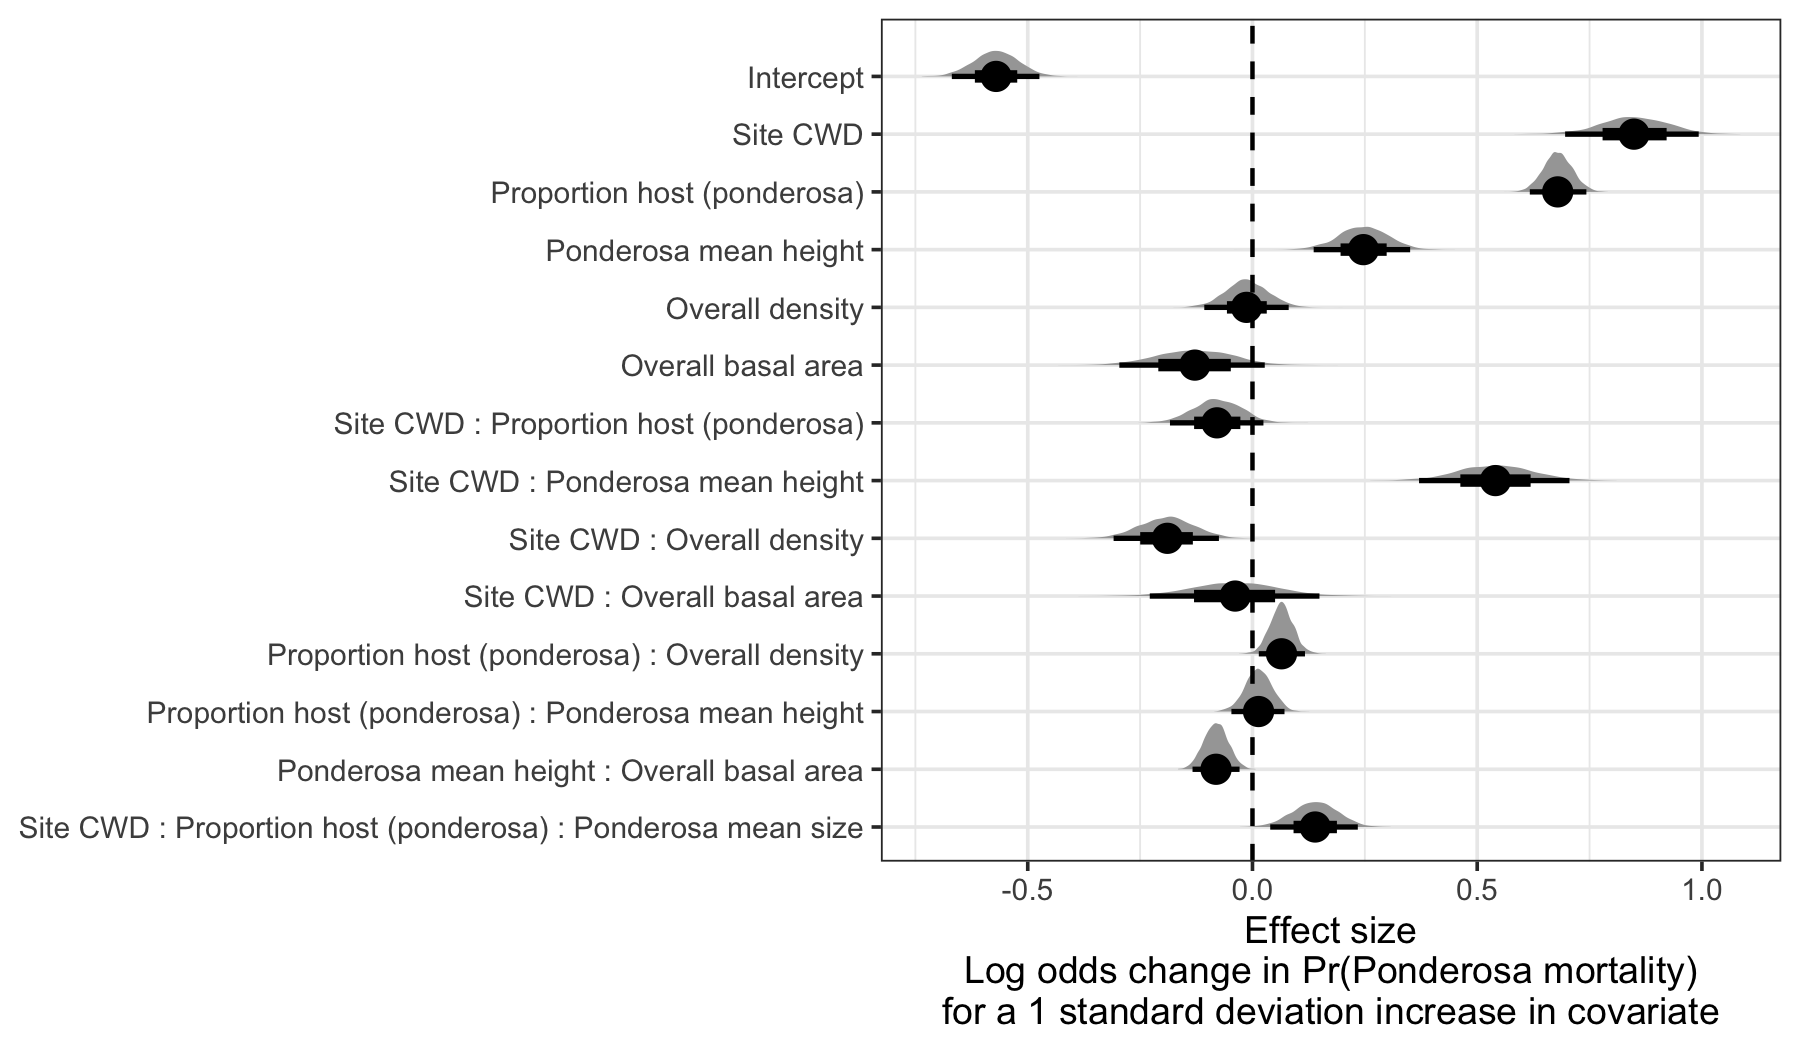
\includegraphics{../../figures/effect-sizes-halfeye.png}
\caption{Posterior distributions of effect size from zero-inflated
binomial model predicting the probability of ponderosa pine mortality in
a 20m x 20m cell given forest structure characteristics of host trees
and all trees within the cell, as well as a site-level climatic water
deficit. The gray density distribution for each model covariate
represents the density of the posterior distribution, the point
underneath each density curve represents the median of the estimate, the
bold interval surrounding the point estimate represents the 66\%
credible interval, and the thin interval surrounding the point estimate
represents the 95\% credible interval.}
\end{figure}

\begin{figure}
\centering
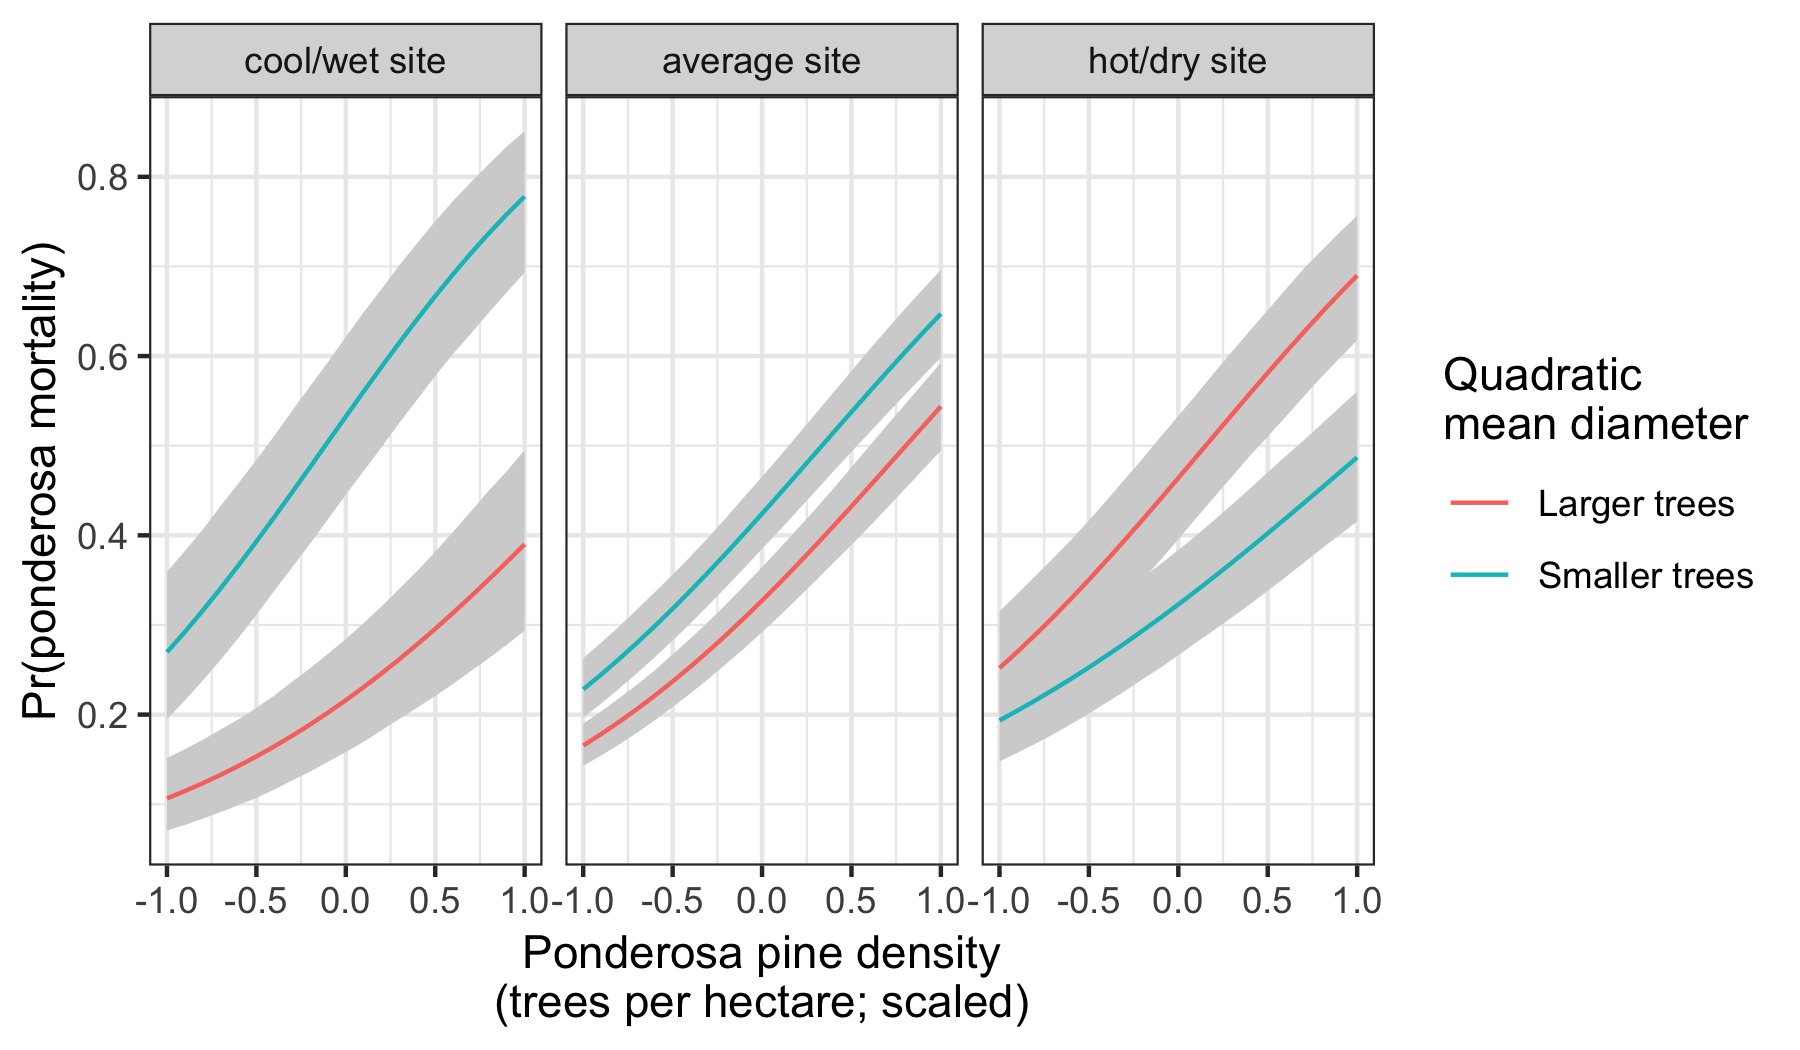
\includegraphics{../../figures/pipo_tpha_qmd_cwd_interaction.png}
\caption{Line version of model results with 95\% credible intervals
showing primary influence of ponderosa pine structure on the probability
of ponderosa pine mortality, and the interaction across climatic water
deficit. The ``larger trees'' line represents the quadratic mean
diameter of ponderosa pine 0.7 standard deviations above the mean, and
the ``smaller trees'' line represents the quadratic mean diameter of
ponderosa pine 0.7 standard deviations below the mean.}
\end{figure}

\subsubsection{Tree detection}\label{tree-detection-1}

We found that the experimental \texttt{lmfx} algorithm with parameter
values of \texttt{dist2d\ =\ 1} and \texttt{ws\ =\ 2.5} (Roussel et al.
2019) performed the best across 7 measures of forest structure as
measured by Pearson's correlation with ground data (Table 3).

\begin{verbatim}
## 
## ----------------------------------------------------------------------------------------------
##    Forest structure metric      Ground mean   Correlation with ground    RMSE    Median error 
## ------------------------------ ------------- ------------------------- -------- --------------
##        total tree count             19                 0.67*            8.68*         2       
## 
##      count of trees > 15m           9.9                0.43              7.38         0       
## 
##  dist to 1st nearest neighbor       2.8                0.55*            1.16*        0.26     
##              (m)                                                                              
## 
##  dist to 2nd nearest neighbor       4.3                0.61*            1.70*        0.12     
##              (m)                                                                              
## 
##  height (m); 25th percentile        12                 0.16              8.46        -1.2     
## 
##        height (m); mean             18                 0.29             7.81*        -2.3     
## 
##  height (m); 75th percentile        25                 0.35             10.33*        -4      
## ----------------------------------------------------------------------------------------------
## 
## Table: Correlation and differences between the best performing tree detection algorithm (lmfx with dist2d = 1 and ws = 2.5) and the ground data. An asterisk next to the correlation or RMSE indicates that this value was within 5% of the value of the best-performing algorithm/parameter set. Ground mean represents the mean value of the forest metric across the 110 ground plots that were visible from the sUAS-derived imagery. The median error is calculated as the median of the differences between the air and ground values for the 110 visible plots. Thus, a positive number indicates an overestimate by the sUAS workflow and a negative number indicates an underestimate.
\end{verbatim}

\subsubsection{Effect of local structure and regional climate on western
pine beetle
severity}\label{effect-of-local-structure-and-regional-climate-on-western-pine-beetle-severity}

We detected no main effect of climatic water deficit on the probability
of ponderosa pine mortality within each 20m x 20m cell.

We found a strong main effect of ponderosa pine local density,
accounting for quadratic mean diameter of ponderosa pine, with greater
density increasing the probability of ponderosa pine mortality.

Conversely, we found a generally negative effect of quadratic mean
diameter of ponderosa pine on the probability of ponderosa mortality,
suggesting that the western pine beetle attacked smaller trees, on
average. There was a strong positive interaction between the climatic
water deficit and ponderosa pine quadratic mean diameter, such that
larger trees were more likely to increase the probability of ponderosa
mortality in hotter, drier sites.

We found negative main effects of overall tree density and overall
quadratic mean diameter. There was a positive interaction between these
variables, such that denser stands with larger trees did lead to greater
ponderosa pine mortality.

\subsubsection{Spatial effects}\label{spatial-effects}

We were able to calculate the length scale of the spatial
autocorrelation in the probability of ponderosa pine mortality at each
site, accounting for forest structure and environmental factors. By
fitting a separate approximate Gaussian process for each site on the
interacting variables of the x- and y- position, we measured the spatial
covariance inherent in the data, accounting for other factors. \#\#
Discussion

\subsubsection{Closer spacing between potential host trees facilitates
dispersal}\label{closer-spacing-between-potential-host-trees-facilitates-dispersal}

If this drives mortality patterns, then we'd expect the local density of
ponderosa pine trees, accounting for other variables, to have a strong
positive effect.

\subsubsection{Host preference for large
trees}\label{host-preference-for-large-trees}

If this drives mortality patterns, then we'd expect the quadratic mean
diameter of ponderosa pine trees, accounting for other variables, to
have a strong positive effect.

\subsubsection{Denser forests augment pheromone
communication}\label{denser-forests-augment-pheromone-communication}

If this drives mortality patterns, then we'd expect the local density of
all trees, accounting for other variables, to have a strong positive
effect.

\subsubsection{Tree crowding leads to greater average water stress per
tree}\label{tree-crowding-leads-to-greater-average-water-stress-per-tree}

If this drives mortality patterns, then we'd expect the quadratic mean
dimater of all trees, accounting for other factors, to have a strong
positive effect.

\subsubsection{Interaction between host density and host
size}\label{interaction-between-host-density-and-host-size}

A positive coefficient would indicate a combined effect of WPB
preference for large trees and nearby host availability.

\subsubsection{Interaction between all tree density and all tree
size}\label{interaction-between-all-tree-density-and-all-tree-size}

A positive coefficient would indicate a combined effect of tree crowding
and pheromone communication enhancement.

\subsubsection{Implications of forest structure/regional climate
interactions}\label{implications-of-forest-structureregional-climate-interactions}

We found that the probability of ponderosa pine mortality generally
increased with local host availability (host density), but also
interacted with both host size and regional climate such that the role
of tree size became increasingly important in more climatically extreme
sites. A smaller average tree size led to a lower probability of
ponderosa mortality in cool/wet sites and a larger average tree size led
to a greater probability of ponderosa mortality in hot/dry sites. These
mortality patterns highlight a possible distinction in behavior between
the recent western bark beetle activity across the gradient of climatic
water deficit. Even in the most highly impacted forest stands (because
our study sites were selected conditional on there being high levels of
western pine beetle activity), there is still a detectable effect of
tree size such that the smaller (presumably weaker) trees are getting
killed in cooler/wetter sites, and the larger (presumably more
well-defended) trees are getting killed more in the hotter/drier sites.
So while mortality is high everywhere, there does appear to be a
difference in the beetle choosiness across the climatic water deficit
gradient.

\subsubsection{Similarities and differences with Fettig et al.
(2019)}\label{similarities-and-differences-with-fettig2019}

Fettig et al. (2019) found positive relationship between number of trees
killed and: total number of trees, total basal area, stand density
index.

Fettig et al. (2019) found negative relationship between the proportion
of trees killed and: total number of trees, stand density index.

Hayes et al. (2009) and Fettig et al. (2019) found measures of host
availability explained less variation in mortality than measures of
stand density.

Negrón et al. (2009) reported positive association of probability of
ponderosa pine mortality and tree density during a drought in Arizona.

Effect of competition may be masked because drought was so extreme
Fettig et al. (2019); Floyd et al. (2009), which is perhaps why we saw a
counter-intuitive signal of increasing total basal area leading to lower
probability of ponderosa pine mortality.

\subsubsection{Broader context around field
plots}\label{broader-context-around-field-plots}

We surveyed 9 square kilometers of forest representing
\textasciitilde{}450,000 trees along a broad environmental gradient of
climatic water deficit. Site selection and small plot size can influence
inference. For instance, Fettig et al. (2019) reported statistically
undetectable differences in overall mortality in their plot network
across 4 national forests. By expanding the hectarage surveyed by a
factor of 200, we detected dramatic differences in overall mortality.

This is about more than sample size (though that helps). This is also
about capturing the local disturbance phenomenon.

\subsubsection{Implications for future forest
structure}\label{implications-for-future-forest-structure}

We have demonstrated that forest structure (local host density and size)
affected the cumulative severity of the western pine beetle in the
Sierra Nevada in the 2012 to 2015 drought and its aftermath. Clearly,
this forest insect disturbance has reciprically impacted the forest
structure, with uncertain consequences for long-term forest dynamics.

Small trees are getting killed in cooler/wetter sites, larger trees
getting killed in hotter/drier sites. Perhaps the cooler/wetter sites
are resisting even this massive disturbance event?

\subsubsection{Spatial effect}\label{spatial-effect}

The western pine beetle is known to exhibit strong aggregation and
anti-aggregation behavior arising from its pheromone communication, and
thus it is likely that the measured spatial covariance in this study is
attributable in part to the magnitude of this effect at each site.

Some studies have suggested that ``outbreak'' conditions are
distinguishable by clustered tree mortality, but this is perhaps
challenging to tease apart (Raffa et al. 2008). Our modeling framework
allows for a joint estimation of the effects of forest structure,
environmental condition, and the spatial effect. This framework would be
enhanced with confidence in individual tree level data, and a lot of it,
along with a strong gradient of environmental conditions and forest
structure.

We won't interpret this measure of contagion, because the uncertainties
in this particular study are too great (tree detection, species
classification, dead trees all assumed to be WPB hosts, didn't account
for topographic effects which could also manifest as part of this
spatial covariance process). We do suggest that this could be a
meaningful and quantifiable means of assessing bark beetle ``stage of
outbreak''.

\subsubsection{Future spatial directions (will cut this; here for now so
I can write it down
elsewhere)}\label{future-spatial-directions-will-cut-this-here-for-now-so-i-can-write-it-down-elsewhere}

Perhaps could also compare relative effect of individual tree spacing
(Voronoi polygon area) with the length scale parameter at a certain site
to get at a similar question. A big voronoi polygon area effect and a
short covariance kernel tells us that it's a water stress effect-- a
crowded tree gets attacked regardless of whether nearby trees were
attacked. A small voronoi polygon area effect and a long covariance
kernel tells us that the mortality is patterned more based on there
being spillover from nearby attacked neighbors instead of how crowded
any given tree is. I expect we might see different relative magnitudes
of voronoi polygon area and covariance kerenel effects depending on CWD.

\subsubsection{Important considerations}\label{important-considerations}

Cumulative effect of elevated insect activity, as mortality was spread
out over 5 years and we surveyed at the end. All the detected dead trees
were considered ponderosa pine-- we know this is wrong. Only about 3 out
of 4 dead trees in Fettig et al. (2019) were ponderosa.

\subsubsection{Room for improvement}\label{room-for-improvement}

\begin{itemize}
\tightlist
\item
  Better geometry by using higher overlap, more spatially resolved
  images.
\item
  Better image classification and scalability by using instrumentation
  having spectral overlap with more widely deployed instrumentation
  (e.g., Landsat).
\item
  Better tree detection using machine learning approaches
\item
  Our live/dead classifier works pretty well.
\item
  Our species classifier could improve. Perhaps also using machine
  learning approaches.
\end{itemize}

(Seidl et al. 2015) (Preisler et al. 2017)

\subsection*{References}\label{references}
\addcontentsline{toc}{subsection}{References}

\hypertarget{refs}{}
\hypertarget{ref-baldwin2017a}{}
Baldwin, B. G., A. H. Thornhill, W. A. Freyman, D. D. Ackerly, M. M.
Kling, N. Morueta-Holme, and B. D. Mishler. 2017. Species richness and
endemism in the native flora of California. American Journal of Botany
104:487--501.

\hypertarget{ref-brooks1998}{}
Brooks, S. P., and A. Gelman. 1998. General Methods for Monitoring
Convergence of Iterative Simulations. Journal of Computational and
Graphical Statistics 7:434.

\hypertarget{ref-burkner2017}{}
Bürkner, P.-C. 2017. \textbf{Brms} : An \emph{R} Package for Bayesian
Multilevel Models Using \emph{Stan}. Journal of Statistical Software 80.

\hypertarget{ref-clevers2013}{}
Clevers, J., and A. Gitelson. 2013. Remote estimation of crop and grass
chlorophyll and nitrogen content using red-edge bands on Sentinel-2 and
-3. International Journal of Applied Earth Observation and
Geoinformation 23:344--351.

\hypertarget{ref-coops2006}{}
Coops, N. C., M. Johnson, M. A. Wulder, and J. C. White. 2006.
Assessment of QuickBird high spatial resolution imagery to detect red
attack damage due to mountain pine beetle infestation. Remote Sensing of
Environment 103:67--80.

\hypertarget{ref-dji2015}{}
DJI. 2015a. Zenmuse X3 - Creativity Unleashed.
\url{https://www.dji.com/zenmuse-x3/info}.

\hypertarget{ref-dji2015a}{}
DJI. 2015b. DJI - The World Leader in Camera Drones/Quadcopters for
Aerial Photography. \url{https://www.dji.com/matrice100/info}.

\hypertarget{ref-dronesmadeeasy2018}{}
Easy, D. M. 2018. ‎Map Pilot for DJI.
\url{https://itunes.apple.com/us/app/map-pilot-for-dji/id1014765000?mt=8}.

\hypertarget{ref-eysn2015}{}
Eysn, L., M. Hollaus, E. Lindberg, F. Berger, J.-M. Monnet, M. Dalponte,
M. Kobal, M. Pellegrini, E. Lingua, D. Mongus, and N. Pfeifer. 2015. A
Benchmark of Lidar-Based Single Tree Detection Methods Using
Heterogeneous Forest Data from the Alpine Space. Forests 6:1721--1747.

\hypertarget{ref-farr2007}{}
Farr, T. G., P. A. Rosen, E. Caro, R. Crippen, R. Duren, S. Hensley, M.
Kobrick, M. Paller, E. Rodriguez, L. Roth, D. Seal, S. Shaffer, J.
Shimada, J. Umland, M. Werner, M. Oskin, D. Burbank, and D. Alsdorf.
2007. The Shuttle Radar Topography Mission. Reviews of Geophysics 45.

\hypertarget{ref-fettig2012b}{}
Fettig, C. J. 2012. Chapter 2: Forest health and bark beetles. \emph{in}
Managing Sierra Nevada Forests. PSW-GTR-237. USDA Forest Service.

\hypertarget{ref-fettig2019}{}
Fettig, C. J., L. A. Mortenson, B. M. Bulaon, and P. B. Foulk. 2019.
Tree mortality following drought in the central and southern Sierra
Nevada, California, U.S. Forest Ecology and Management 432:164--178.

\hypertarget{ref-flint2013}{}
Flint, L. E., A. L. Flint, J. H. Thorne, and R. Boynton. 2013.
Fine-scale hydrologic modeling for regional landscape applications: The
California Basin Characterization Model development and performance.
Ecological Processes 2:25.

\hypertarget{ref-floyd2009}{}
Floyd, M. L., M. Clifford, N. S. Cobb, D. Hanna, R. Delph, P. Ford, and
D. Turner. 2009. Relationship of stand characteristics to
drought-induced mortality in three Southwestern piñonJuniper woodlands.
Ecological Applications 19:1223--1230.

\hypertarget{ref-gabry2019}{}
Gabry, J., D. Simpson, A. Vehtari, M. Betancourt, and A. Gelman. 2019.
Visualization in Bayesian workflow. Journal of the Royal Statistical
Society: Series A (Statistics in Society) 182:389--402.

\hypertarget{ref-gitelson1994}{}
Gitelson, A., and M. N. Merzlyak. 1994. Spectral Reflectance Changes
Associated with Autumn Senescence of Aesculus hippocastanum L. and Acer
platanoides L. Leaves. Spectral Features and Relation to Chlorophyll
Estimation. Journal of Plant Physiology 143:286--292.

\hypertarget{ref-hayes2009}{}
Hayes, C. J., C. J. Fettig, and L. D. Merrill. 2009. Evaluation of
Multiple Funnel Traps and Stand Characteristics for Estimating Western
Pine Beetle-Caused Tree Mortality. Journal of Economic Entomology
102:2170--2182.

\hypertarget{ref-hijmans2019}{}
Hijmans, R. J., J. van Etten, M. Sumner, J. Cheng, A. Bevan, R. Bivand,
L. Busetto, M. Canty, D. Forrest, A. Ghosh, D. Golicher, J. Gray, J. A.
Greenberg, P. Hiemstra, I. for M. A. Geosciences, C. Karney, M.
Mattiuzzi, S. Mosher, J. Nowosad, E. Pebesma, O. P. Lamigueiro, E. B.
Racine, B. Rowlingson, A. Shortridge, B. Venables, and R. Wueest. 2019.
Raster: Geographic Data Analysis and Modeling.

\hypertarget{ref-hunziker2017}{}
Hunziker, P. 2017. Velox: Fast Raster Manipulation and Extraction.

\hypertarget{ref-jakubowski2013}{}
Jakubowski, M. K., W. Li, Q. Guo, and M. Kelly. 2013. Delineating
Individual Trees from Lidar Data: A Comparison of Vector- and
Raster-based Segmentation Approaches. Remote Sensing 5:4163--4186.

\hypertarget{ref-kane2014}{}
Kane, V. R., M. P. North, J. A. Lutz, D. J. Churchill, S. L. Roberts, D.
F. Smith, R. J. McGaughey, J. T. Kane, and M. L. Brooks. 2014. Assessing
fire effects on forest spatial structure using a fusion of Landsat and
airborne LiDAR data in Yosemite National Park. Remote Sensing of
Environment 151:89--101.

\hypertarget{ref-kuhn2008}{}
Kuhn, M. 2008. Building Predictive Models in R Using the caret Package.
Journal of Statistical Software 28:1--26.

\hypertarget{ref-larson2012}{}
Larson, A. J., and D. Churchill. 2012. Tree spatial patterns in
fire-frequent forests of western North America, including mechanisms of
pattern formation and implications for designing fuel reduction and
restoration treatments. Forest Ecology and Management 267:74--92.

\hypertarget{ref-li2012}{}
Li, W., Q. Guo, M. K. Jakubowski, and M. Kelly. 2012. A New Method for
Segmenting Individual Trees from the Lidar Point Cloud. Photogrammetric
Engineering \& Remote Sensing 78:75--84.

\hypertarget{ref-meyer1990}{}
Meyer, F., and S. Beucher. 1990. Morphological segmentation. Journal of
Visual Communication and Image Representation 1:21--46.

\hypertarget{ref-micasense2015}{}
Micasense. 2015. MicaSense.
\url{https://support.micasense.com/hc/en-us/articles/215261448-RedEdge-User-Manual-PDF-Download-}.

\hypertarget{ref-millar2015}{}
Millar, C. I., and N. L. Stephenson. 2015. Temperate forest health in an
era of emerging megadisturbance. Science 349:823--826.

\hypertarget{ref-morris2017}{}
Morris, J. L., S. Cottrell, C. J. Fettig, W. D. Hansen, R. L. Sherriff,
V. A. Carter, J. L. Clear, J. Clement, R. J. DeRose, J. A. Hicke, P. E.
Higuera, K. M. Mattor, A. W. R. Seddon, H. T. Seppä, J. D. Stednick, and
S. J. Seybold. 2017. Managing bark beetle impacts on ecosystems and
society: Priority questions to motivate future research. Journal of
Applied Ecology 54:750--760.

\hypertarget{ref-negron2009}{}
Negrón, J. F., J. D. McMillin, J. A. Anhold, and D. Coulson. 2009. Bark
beetle-caused mortality in a drought-affected ponderosa pine landscape
in Arizona, USA. Forest Ecology and Management 257:1353--1362.

\hypertarget{ref-north2015}{}
North, M. P., S. L. Stephens, B. M. Collins, J. K. Agee, G. Aplet, J. F.
Franklin, and P. Z. Fule. 2015. Reform forest fire management. Science
349:1280--1281.

\hypertarget{ref-pau2010}{}
Pau, G., F. Fuchs, O. Sklyar, M. Boutros, and W. Huber. 2010. EBImagean
R package for image processing with applications to cellular phenotypes.
Bioinformatics 26:979--981.

\hypertarget{ref-pebesma2019}{}
Pebesma, E., R. Bivand, E. Racine, M. Sumner, I. Cook, T. Keitt, R.
Lovelace, H. Wickham, J. Ooms, K. Müller, and T. L. Pedersen. 2019. Sf:
Simple Features for R.

\hypertarget{ref-plowright2018}{}
Plowright, A. 2018. ForestTools: Analyzing Remotely Sensed Forest Data.

\hypertarget{ref-popescu2004}{}
Popescu, S. C., and R. H. Wynne. 2004. Seeing the Trees in the Forest:
Using Lidar and Multispectral Data Fusion with Local Filtering and
Variable Window Size for Estimating Tree Height. PHOTOGRAMMETRIC
ENGINEERING:16.

\hypertarget{ref-preisler2017}{}
Preisler, H. K., N. E. Grulke, Z. Heath, and S. L. Smith. 2017. Analysis
and out-year forecast of beetle, borer, and drought-induced tree
mortality in California. Forest Ecology and Management. 399: 166-178
399:166--178.

\hypertarget{ref-rcoreteam2018}{}
R Core Team. 2018. R: A Language and Environment for Statistical
Computing. R Foundation for Statistical Computing, Vienna, Austria.

\hypertarget{ref-raffa2008}{}
Raffa, K. F., B. H. Aukema, B. J. Bentz, A. L. Carroll, J. A. Hicke, M.
G. Turner, and W. H. Romme. 2008. Cross-scale Drivers of Natural
Disturbances Prone to Anthropogenic Amplification: The Dynamics of Bark
Beetle Eruptions. BioScience 58:501--517.

\hypertarget{ref-raffa2015}{}
Raffa, K. F., J.-C. Grégoire, and B. Staffan Lindgren. 2015. Natural
History and Ecology of Bark Beetles. Pages 1--40 \emph{in} Bark Beetles.
Elsevier.

\hypertarget{ref-rouse1973}{}
Rouse, W., R. H. Haas, W. Deering, and J. A. Schell. 1973. MONITORING
THE VERNAL ADVANCEMENT AND RETROGRADATION (GREEN WAVE EFFECT) OF NATURAL
VEGETATION. Type II Report, Goddard Space Flight Center, Greenbelt, MD,
USA.

\hypertarget{ref-roussel2019a}{}
Roussel, J.-R. 2019. lidRplugins: Extra functions and algorithms for
lidR package.

\hypertarget{ref-roussel2019}{}
Roussel, J.-R., D. A. (. the documentation), F. D. B. (. bugs and
improved catalog features), and A. S. M. (. lassnags). 2019. lidR:
Airborne LiDAR Data Manipulation and Visualization for Forestry
Applications.

\hypertarget{ref-seidl2015}{}
Seidl, R., J. Müller, T. Hothorn, C. Bässler, M. Heurich, and M. Kautz.
2015. Small beetle, large-scale drivers: How regional and landscape
factors affect outbreaks of the European spruce bark beetle. The Journal
of applied ecology 53:530--540.

\hypertarget{ref-shiklomanov2019}{}
Shiklomanov, A. N., B. A. Bradley, K. M. Dahlin, A. M. Fox, C. M. Gough,
F. M. Hoffman, E. M. Middleton, S. P. Serbin, L. Smallman, and W. K.
Smith. 2019. Enhancing global change experiments through integration of
remote-sensing techniques. Frontiers in Ecology and the Environment 0.

\hypertarget{ref-shin2018}{}
Shin, P., T. Sankey, M. Moore, and A. Thode. 2018. Evaluating Unmanned
Aerial Vehicle Images for Estimating Forest Canopy Fuels in a Ponderosa
Pine Stand. Remote Sensing 10:1266.

\hypertarget{ref-stephenson1998}{}
Stephenson, N. 1998. Actual evapotranspiration and deficit: Biologically
meaningful correlates of vegetation distribution across spatial scales.
Journal of Biogeography 25:855--870.

\hypertarget{ref-stephenson2019}{}
Stephenson, N. L., A. J. Das, N. J. Ampersee, and B. M. Bulaon. 2019.
Which trees die during drought? The key role of insect host-tree
selection. Journal of Ecology:75.

\hypertarget{ref-usdafs2019}{}
USDAFS. 2019, February 11. Press Release: Survey finds 18 million trees
died in California in 2018.
\url{https://www.fs.usda.gov/Internet/FSE_DOCUMENTS/FSEPRD609321.pdf}.

\hypertarget{ref-vega2014}{}
Vega, C., A. Hamrouni, S. El Mokhtari, J. Morel, J. Bock, J. P. Renaud,
M. Bouvier, and S. Durrieu. 2014. PTrees: A point-based approach to
forest tree extraction from lidar data. International Journal of Applied
Earth Observation and Geoinformation 33:98--108.

\hypertarget{ref-young2017}{}
Young, D. J. N., J. T. Stevens, J. M. Earles, J. Moore, A. Ellis, A. L.
Jirka, and A. M. Latimer. 2017. Long-term climate and competition
explain forest mortality patterns under extreme drought. Ecology Letters
20:78--86.

\hypertarget{ref-zhang2016}{}
Zhang, W., J. Qi, P. Wan, H. Wang, D. Xie, X. Wang, and G. Yan. 2016. An
Easy-to-Use Airborne LiDAR Data Filtering Method Based on Cloth
Simulation. Remote Sensing 8:501.


\end{document}
